\documentclass[10pt,a4paper]{beamer}
\usepackage[latin1]{inputenc}
\usepackage[spanish]{babel}
\usepackage[T1]{fontenc}
\usepackage{amsmath}
\usepackage{amsfonts}
\usepackage{amssymb}
\usepackage{graphicx}
\usepackage{beamerthemesplit}
\usepackage{float}
\usepackage{multirow}
\usepackage{multicol}
\usepackage{url}
\usepackage{ragged2e}
\usepackage{array}
\usepackage{latexsym}
\usepackage{subfigure}
\usepackage{timing}
\usepackage{url}

\setbeamertemplate{footline}[frame number]
\setbeamertemplate{bibliography item}[text]
%\setbeamertemplate{subsubsection in sidebar shaded}
%{\tableofcontents[subsubsectionstyle=hide]}

%\usetheme{Montpellier}
\usetheme{Warsaw}
\decimalpoint
\renewcommand{\contentsname}{Contenido}

\begin{document}

\title{Integraci�n sem�ntica de \\ los recursos de informaci�n en \\ una memoria corporativa}
\author{Erik Alarc�n Zamora}
\date{Enero 2014. M�xico, D.F.}

\begin{frame}
\titlepage
\centering
Asesores:\\ Dra. Reyna Carolina Medina Ram�rez \\Dr. H�ctor P�rez Urbina
\\
\end{frame}
\begin{frame}
\frametitle{Contenido}
\setcounter{tocdepth}{1}  
\begin{scriptsize}\tableofcontents[]\end{scriptsize}
\end{frame}
\section{Contexto y motivaci�n}

\subsection{Memoria corporativa}
\begin{frame}
	\frametitle{Memoria Corporativa}
	%%%%%%%%%%%%%%%%%%%%%%%
	\begin{block}{Definici�n}
	\justifying 
	La representaci�n expl�cita, t�cita, consistente y persistente del conocimiento de una organizaci�n. \cite{Ontoinra2002}
	\end{block}
	
	\begin{figure}[htbp]
	\centering
	\subfigure{
	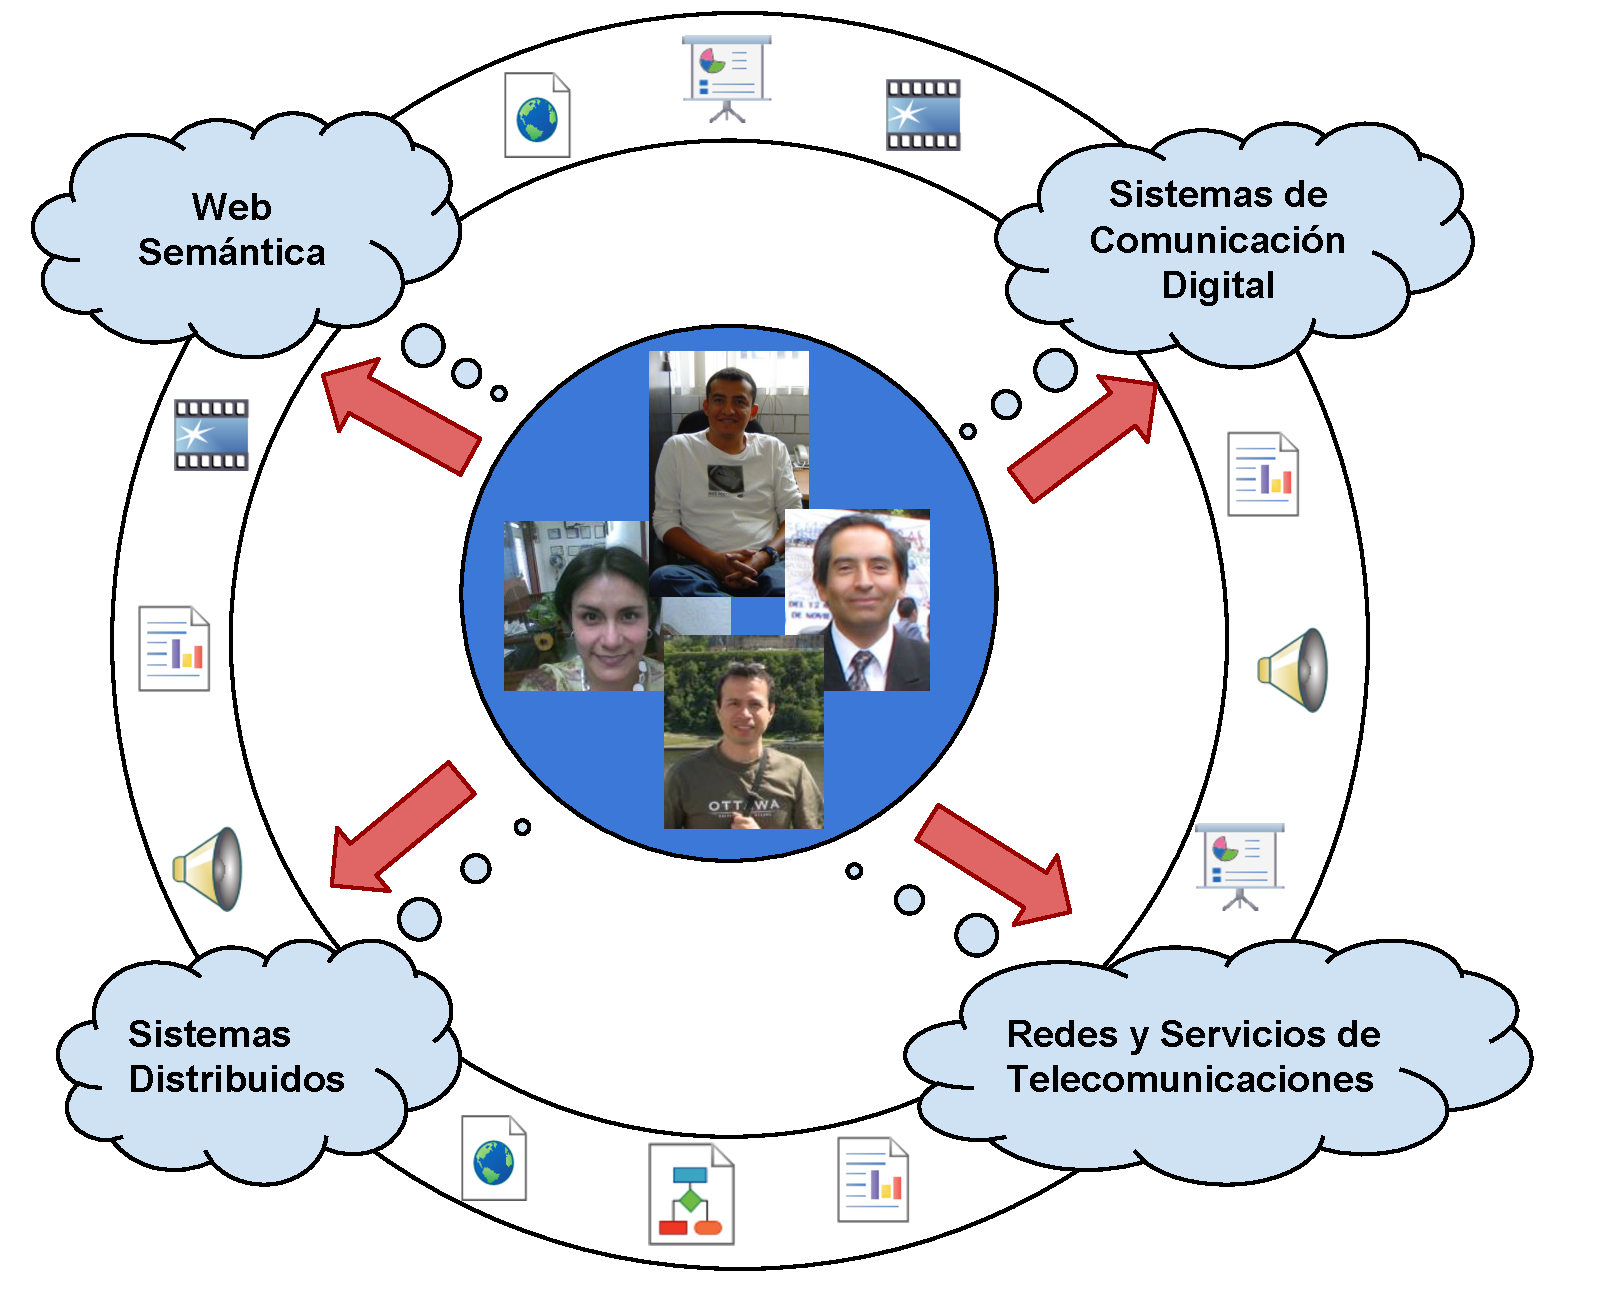
\includegraphics[scale=0.18]{ConocimientoRyT} 
	}
	\subfigure{
	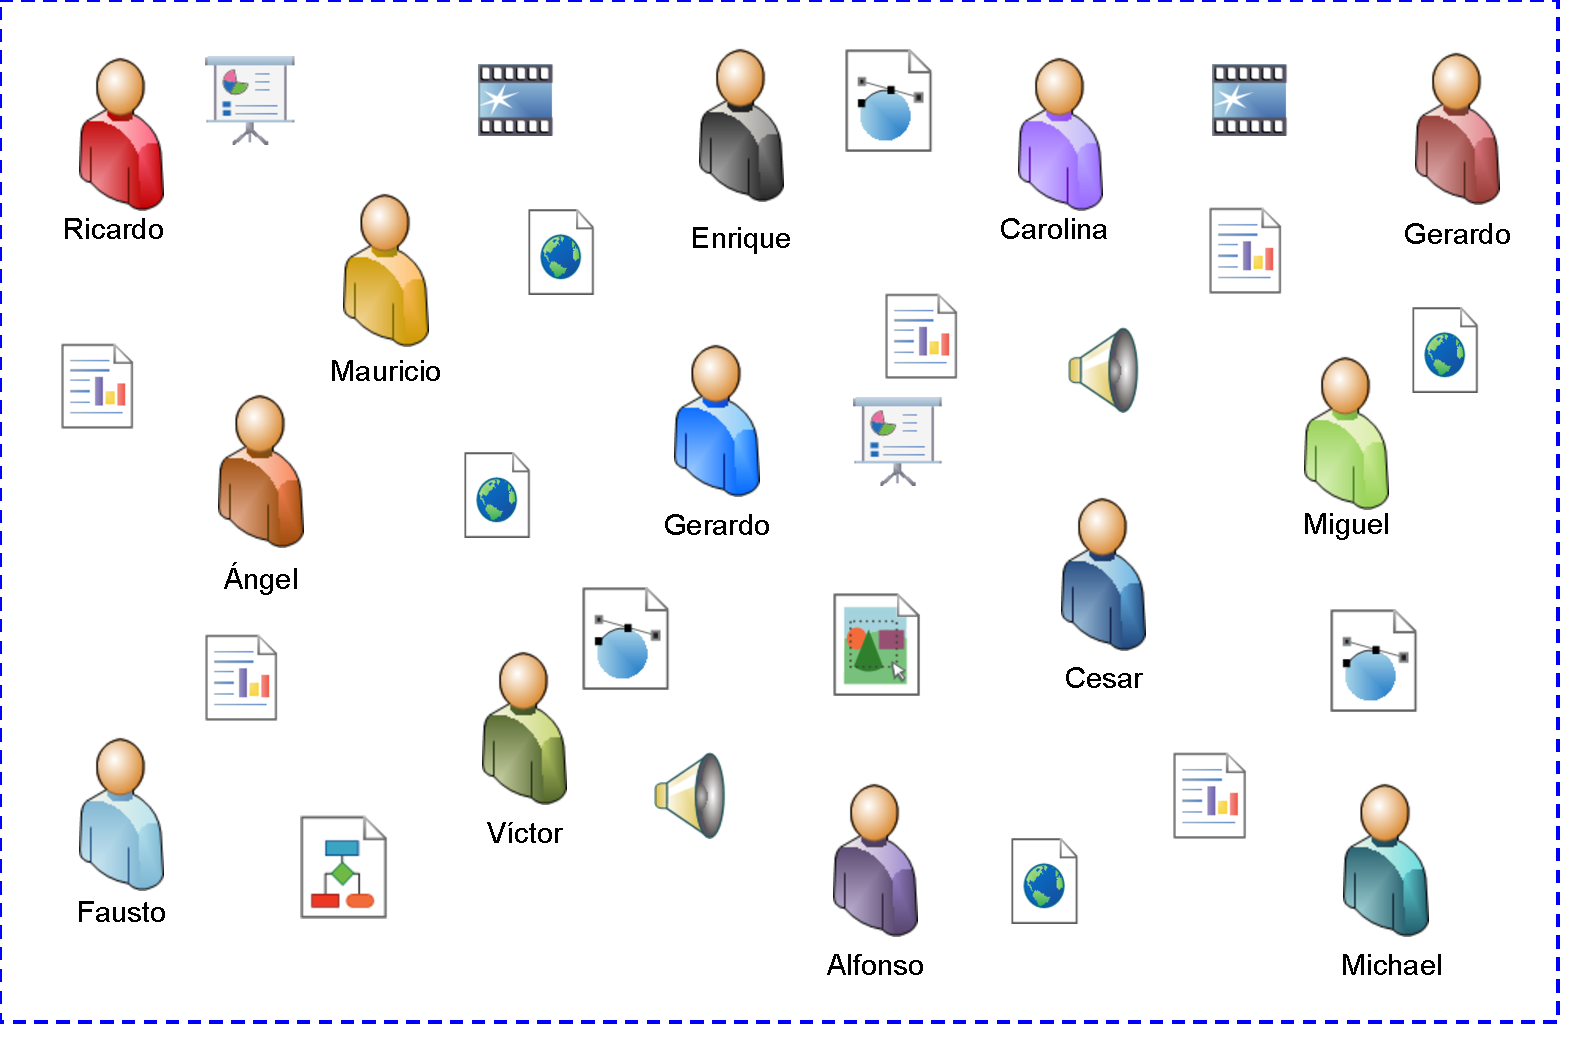
\includegraphics[scale=0.19]{EjemploMC} 
	}
	\end{figure}
	%%%%%%%%%%%%%%%%%%%%%%%
\end{frame}

\subsection{Integraci�n de la informaci�n de los recursos de informaci�n}
\begin{frame}
	\frametitle{Integraci�n de la informaci�n de los recursos de informaci�n}
	\begin{block}{Definici�n}
	\justifying
	\small La b�squeda y recuperaci�n significativa de informaci�n existente en los recursos de informaci�n para responder una consulta dada por un usuario.
	\end{block}
	
	\begin{exampleblock}{Etapas}
	\begin{enumerate}[<+-| alert@+>]
	\item \justifying \small Representar el conocimiento e informaci�n de los \textit{recursos de informaci�n}.
	\item \justifying \small Buscar y recuperar informaci�n, mediante la interrogaci�n de la representaci�n de conocimiento (modelo).
	\end{enumerate}
	\end{exampleblock}
	
	\begin{figure}
	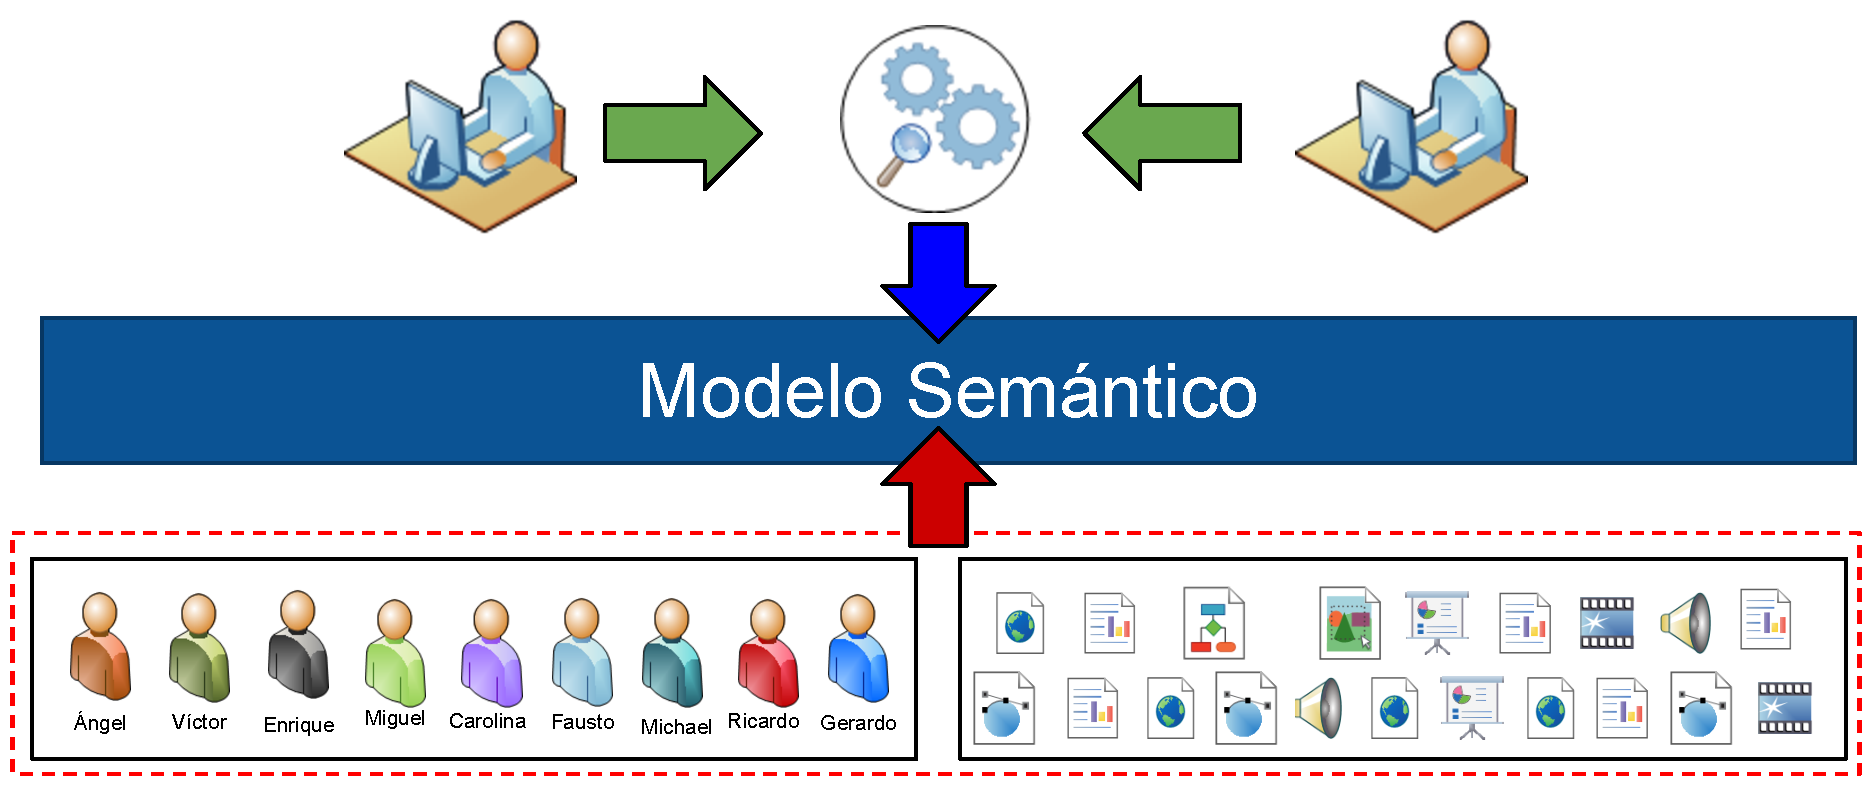
\includegraphics[scale=0.24]{IntegracionSemantica} 
	\end{figure}
\end{frame}

\subsection{Tecnolog�as Sem�nticas}
\begin{frame}
	\frametitle{Tecnolog�as Sem�nticas}
	\begin{block}{Definici�n}
	\justifying 
	\textit{Un conjunto de metodolog�as, lenguajes, aplicaciones, herramientas y est�ndares para suministrar u obtener el significado de las palabras, informaci�n y las relaciones entre �stos}. \begin{scriptsize}\cite{SemTecRetr}\end{scriptsize}
	\end{block}
	
	\begin{figure}
	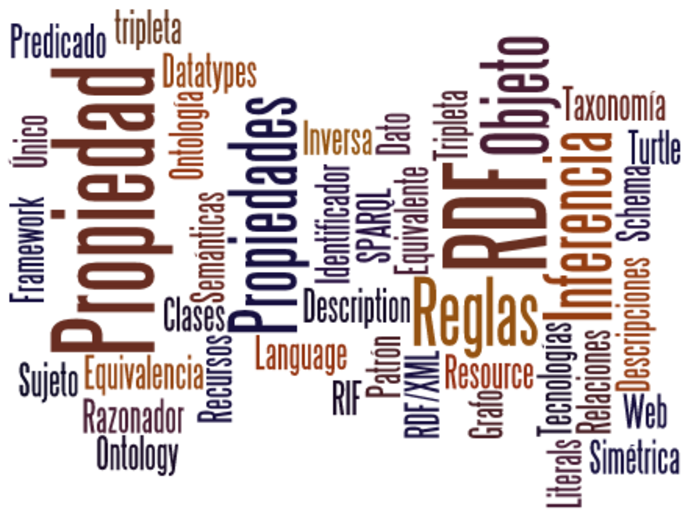
\includegraphics[scale=0.42]{TSWords} 
	\end{figure}
\end{frame}

\subsection{Integraci�n sem�ntica de recursos de informaci�n}
\begin{frame}
	\frametitle{Integraci�n sem�ntica de recursos de informaci�n}
	\begin{figure}
	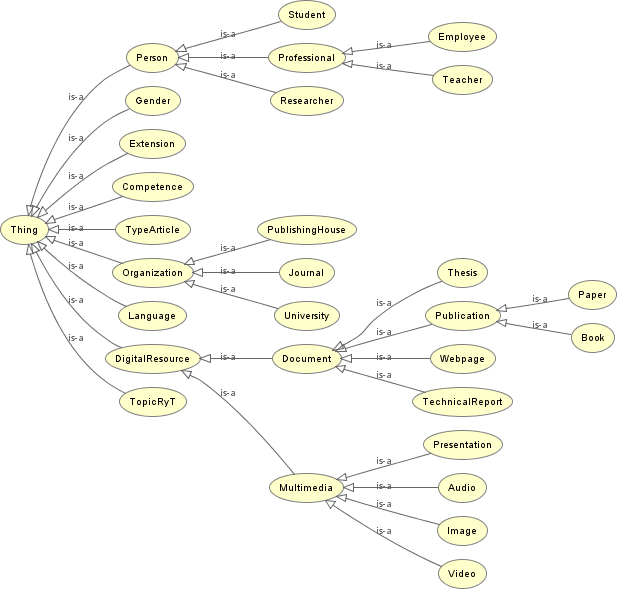
\includegraphics[scale=0.38]{ISRIMC} 
	\end{figure}
\end{frame}

\subsection{Estado del Arte}
\begin{frame}
	\frametitle{Estado del Arte}
	\begin{block}{Ejes claves}
	\begin{enumerate}
	\item \justifying Integraci�n de la informaci�n a partir del uso de tecnolog�as sem�nticas.
	\item \justifying B�squeda, recuperaci�n y publicaci�n de la informaci�n desde una ontolog�a.
	\item \justifying Gesti�n de una memoria corporativa.
	\end{enumerate}
	\end{block}
	
	\begin{figure}
	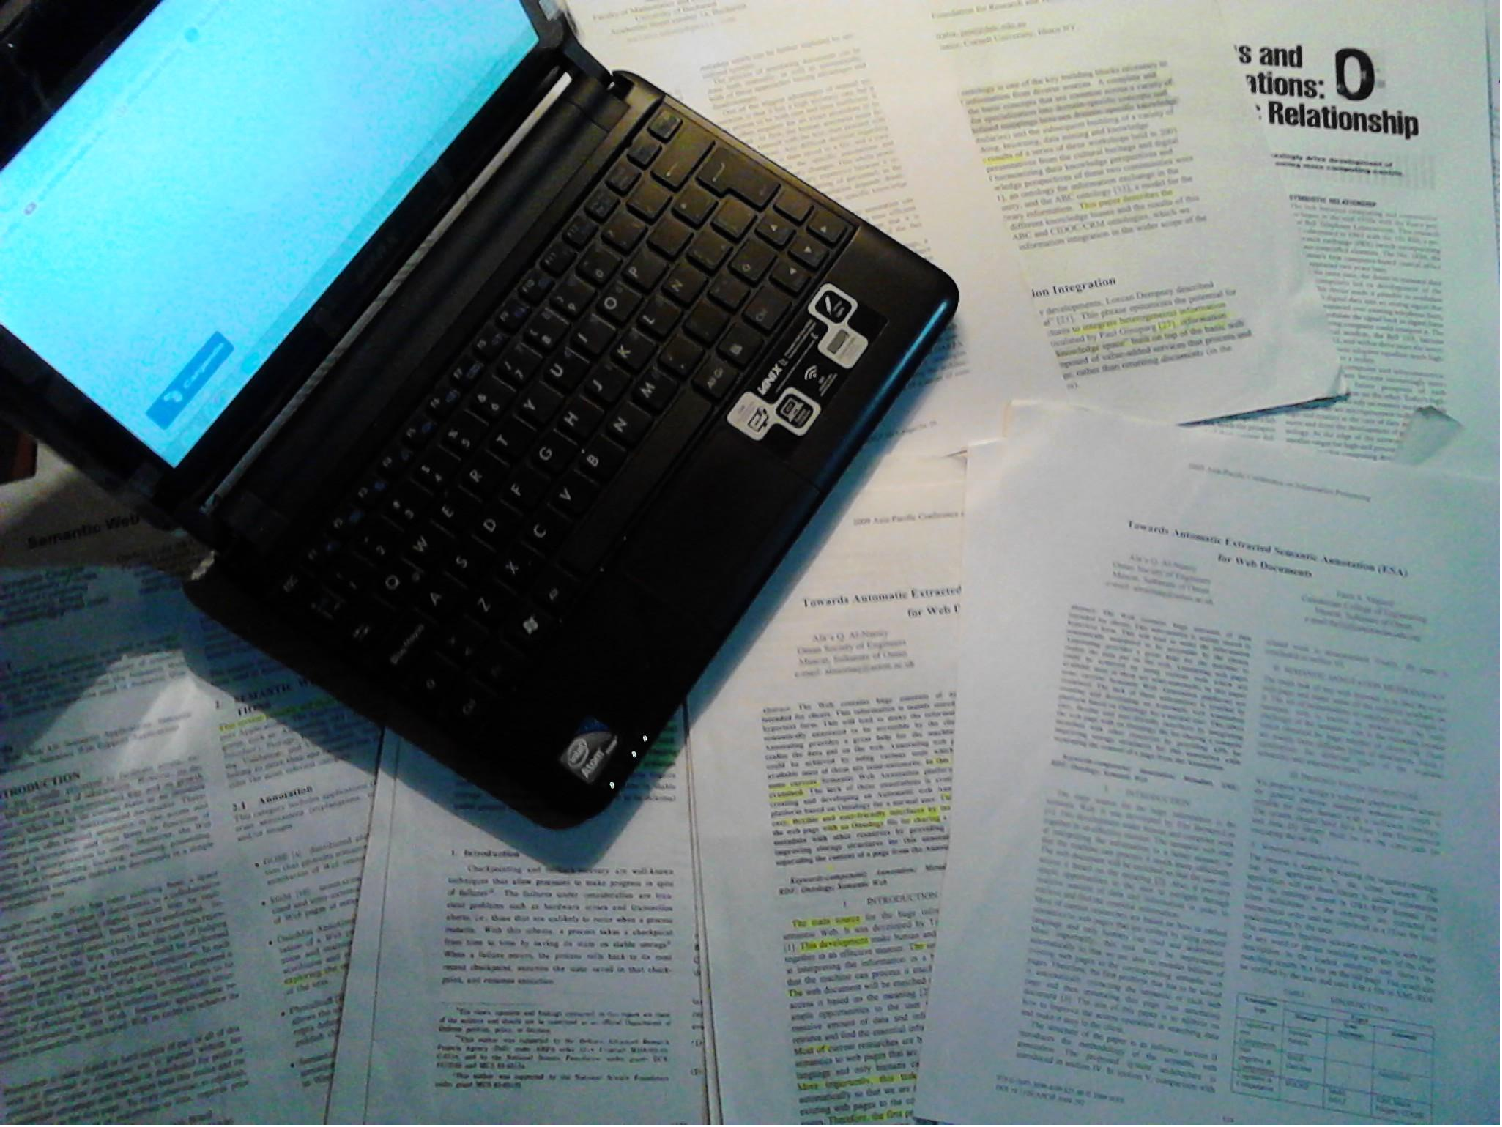
\includegraphics[scale=0.15]{EstadoArte} 
	\end{figure}
\end{frame}

\begin{frame}
	\frametitle{Comparativa}
	\begin{figure}
	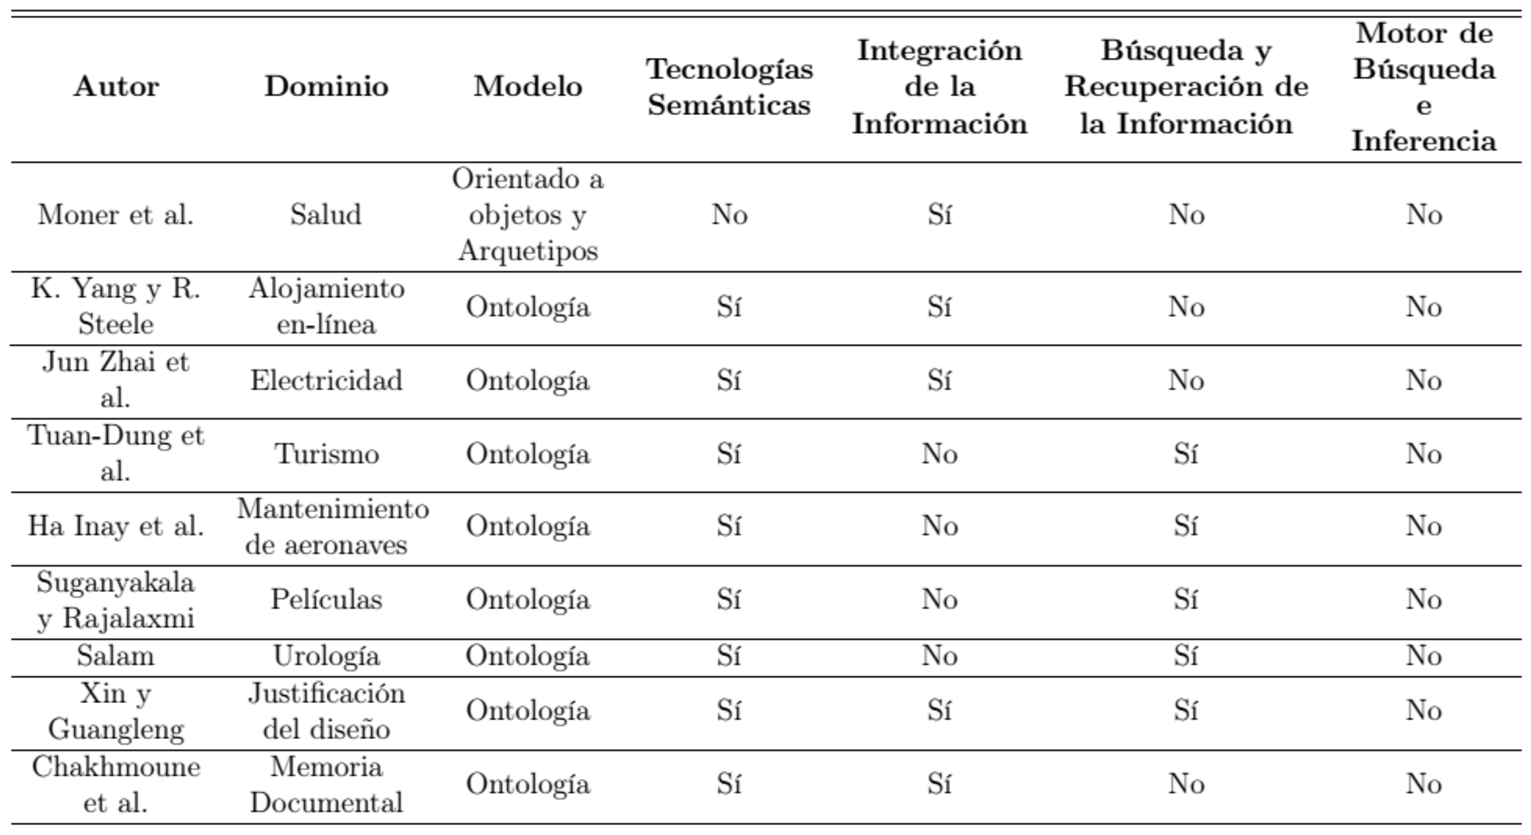
\includegraphics[scale=0.42]{TablaEOA} 
	\end{figure}
\end{frame}
\section{Descripci�n del Problema}

\subsection{Pregunta Investigaci�n}
\begin{frame}
	\frametitle{Pregunta Investigaci�n} 
	\begin{exampleblock}{}
	\justifying 
	\textit{�Las \textbf{tecnolog�as sem�nticas} son viables para solucionar la \textbf{integraci�n sem�ntica} de los \textbf{recursos de informaci�n} de una \textbf{memoria corporativa}?}
	\end{exampleblock}
	
	\begin{figure}
	
\includegraphics[scale=0.4]{PreguntaInv} 
	\end{figure}
\end{frame}

\subsection{Objetivos}
\begin{frame}
	\frametitle{Objetivos} 
	\begin{alertblock}{Objetivo Principal}
	\justifying 
	Contribuir a la \textit{integraci�n sem�ntica} de los \textit{recursos de informaci�n} en \textit{una memoria corporativa}, mediante el uso de las \textit{tecnolog�as sem�nticas}.
	\end{alertblock}
	
	\begin{block}{Objetivos Particulares}
	\begin{enumerate}
	\item \justifying \small Un \textbf{\textit{marco de referencia}} para la \textit{integraci�n sem�ntica} de los \textit{recursos de informaci�n}.
	\item \justifying \small Un \textbf{\textit{modelo sem�ntico}} que representa el \textit{conocimiento expl�cito e impl�cito} de los \textit{recursos de informaci�n}.
	\item \justifying \small Un \textbf{\textit{prototipo de interfaz gr�fica de usuario}} que permita a los usuarios consultar y visualizar la informaci�n de los recursos de informaci�n, interrogando un modelo sem�ntico.
	\item \justifying \small La evaluaci�n de la calidad de los \textbf{\textit{resultados recuperados}} y los \textbf{\textit{tiempos de procesamiento}} de la \textit{integraci�n sem�ntica}.
	\end{enumerate}
	\end{block}
\end{frame}

\subsection{Metodolog�a}
\begin{frame}
	\frametitle{Metodolog�a I}
	\begin{block}{Marco de Referencia}
	\begin{enumerate}
	\item \justifying \small Identificar los \textit{casos de uso}.
	\item \justifying \small Evaluar las \textit{herramientas sem�nticas}.
	\item \justifying \small Conformar los \textit{recurso de informaci�n} de la \textit{memoria corporativa}.
	\end{enumerate}
	
	\begin{exampleblock}{Modelo Sem�ntico}
	\begin{enumerate}
	\setcounter{enumi}{3}
	\item \justifying \small Representar el \textit{conocimiento expl�cito} de los \textit{recursos de informaci�n} en un \textit{modelo sem�ntico} (ontolog�a).
	\item \justifying \small Enriquecer el \textit{modelo sem�ntico} con \textit{reglas de inferencia}.
	\end{enumerate}
	\end{exampleblock}
	
	\begin{enumerate}
	\setcounter{enumi}{5}
	\item \justifying \small Escribir las principales \textit{consultas} en la sintaxis correspondiente.
	\item \justifying \small Emplear un razonador para hacer expl�cito el conocimiento impl�cito.
	\item \justifying \small Buscar y recuperar informaci�n en la memoria corporativa, interrogando el modelo sem�ntico inferido.
	\end{enumerate}
	\end{block}
\end{frame}

\begin{frame}
	\frametitle{Metodolog�a II}	
	\begin{block}{Prototipo de interfaz gr�fica de usuario}	
	\begin{enumerate}
	\setcounter{enumi}{8}
	\item \justifying \small Construir el \textit{prototipo de interfaz de usuario} para la (b�squeda y navegaci�n) de los usuarios en un modelo sem�ntico.
	\end{enumerate}
	\end{block}
	
	\begin{block}{Evaluaci�n}
	\begin{enumerate}
	\setcounter{enumi}{9}
	\item \justifying \small Evaluar la calidad de los resultados con y sin inferencia.
	\item \justifying \small Evaluar los \textit{tiempos promedios} de consulta sobre modelos con/sin inferencia.
	\end{enumerate}
	\end{block}
\end{frame}

\subsection{Hip�tesis}
\begin{frame}
	\frametitle{Hip�tesis}
	\begin{block}{}
	\justifying 
	\textbf{El uso de las \textit{tecnolog�as sem�nticas} es adecuado para lograr la \textit{integraci�n sem�ntica} de \textit{recursos de informaci�n} en una \textit{memoria corporativa}}.
	\end{block}
	
	\begin{figure}
	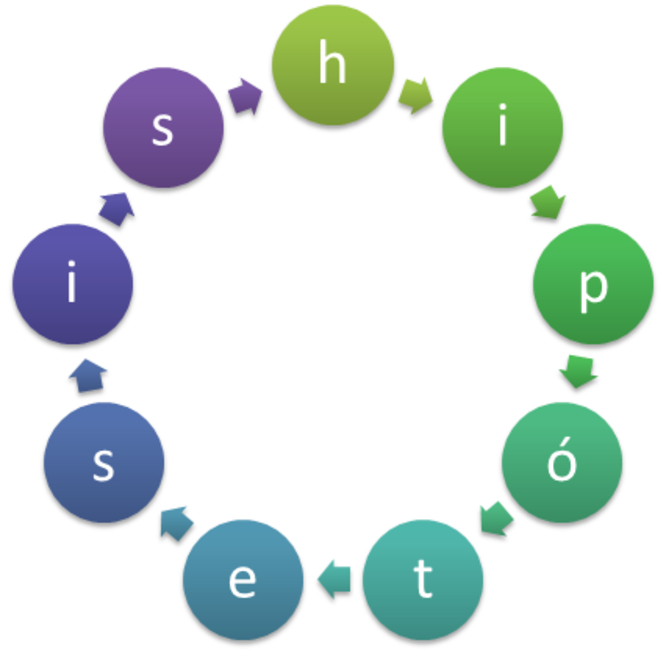
\includegraphics[scale=0.45]{hipotesis} 
	\end{figure}
\end{frame}

\subsection{Aportaciones}
\begin{frame}
	\frametitle{Aportaciones}
	\begin{enumerate}
	\item \justifying Un \textit{marco de referencia} para lograr la \textit{integraci�n sem�ntica} de \textit{recursos de informaci�n}.
    \item \justifying Un modelo sem�ntico que representa el conocimiento de una memoria corporativa.
    \item \justifying  Un prototipo (interfaz gr�fica de usuario) para la interacci�n amigable (b�squeda y consulta de informaci�n) de los usuarios con el modelo sem�ntico.
    \item \justifying Los resultados de nuestra evaluaci�n experimental.
    \item \justifying Un par de scripts para la generaci�n autom�tica y controlada de descripciones (conocimiento expl�cito) de los \textit{recursos de informaci�n}.
	\end{enumerate}
\end{frame}
%%%%%%%%%%%%%%%%%%%%%%%%%%%%%%%%%%%%%%%%%%%%%%%%%%%%%%%%%%%%%%%%%%%%%%%%%%%%%%
\chapter{Estado del arte}
\label{cap:soa}
La \textbf{\textit{integraci�n de los recursos de informaci�n en una memoria corporativa}} ha sido poco explotada por las organizaciones o �reas de investigaci�n. Existen algunos trabajos sobre la \textit{integraci�n de informaci�n} que incorporan a las tecnolog�as sem�nticas para representar y enriquecer el conocimiento de un dominio dado, as� como, la b�squeda de informaci�n a partir de este conocimiento. Los trabajos para este \textit{estado del arte}, son aquellos que cumplen con alguno de estos criterios:

\begin{itemize}
\item Integraci�n de los recursos: es el proceso de b�squeda y recuperaci�n de la informaci�n sobre los recursos de informaci�n. En la secci�n \ref{sec:intdk} se define formalmente este concepto.
\item Memoria corporativa: es la representaci�n del conocimiento en una organizaci�n. En la secci�n \ref{sec:mecor} se define formalmente este concepto.
\item Modelo sem�ntico: es la representaci�n del conocimiento a partir de las tecnolog�as sem�nticas. En la secci�n \ref{sec:rdf} y \ref{sec:reginf} se describe este concepto.
\item Inferencia en el modelo: es el proceso de deducir informaci�n a partir del modelo sem�ntico. En la secci�n \ref{sec:reginf} se define formalmente este concepto.
\item Interfaz de usuario: es la construcci�n de un aplicaci�n visual para que los usuarios pregunten o naveguen a partir  del modelo sem�ntico. En la secci�n \ref{cap:piu} se describen las funciones que debe tener un prototipo para la integraci�n de los recursos.
\end{itemize}

La secci�n \label{sec:eoaisr} describe los trabajos que se estudiaron para la integraci�n de los recursos. Al final de esta secci�n, se presenta una tabla comparativa de estos trabajos y los criterios que �stos cumplen.

En este \textit{estado del arte} se contempla un estudio de las aplicaciones para realizar la \textit{integraci�n sem�ntica de los recursos en una memoria corporativa}. Las aplicaciones estudiadas, se agrupan de acuerdo a las siguientes funcionalidades.

\begin{enumerate}
\item Escribir los declaraciones en forma de triple y guardarlos en alguna sintaxis est�ndar.
\item Escribir los axiomas mediante los vocabularios est�ndar (OWL y RDF(S)).
\item Gesti�n del grafo RDF, es decir, carga del modelo, consulta de informaci�n e inferencia.
\end{enumerate}

En la secci�n \ref{sec:eoats}, se describen estas aplicaciones con base en su funcionalidad. Al final de cada agrupaci�n, se da a conocer: \textit{cu�l herramienta se eligi� para facilitar y efectuar la funcionalidad dada}.

\section{Integraci�n sem�ntica de recursos de informaci�n}
\label{sec:eoaisr}
El principal objetivo de la integraci�n de los recursos es buscar y recuperar informaci�n significativa que est� en los recursos, para responder las necesidades informativas de las personas. Una integraci�n sem�ntica de recursos emplea las tecnolog�as sem�nticas con la finalidad de recuperar informaci�n m�s significativa en los recursos a partir de las caracter�sticas y relaciones de estos. El uso de una memoria corporativa para la integraci�n sem�ntica, se traduce en informaci�n y conocimiento de los recursos bajo un dominio particular.

Algunos trabajos exploran o emplean el enfoque sem�ntico para fines de integraci�n del conocimiento, representaci�n de una memoria corporativa o b�squeda de informaci�n. A continuaci�n, se describe el estado actual del conocimiento referente a estos trabajos.

La \textbf{\textit{arquitectura del modelo dual}} \cite{Archetype} es una propuesta para la representaci�n consistente y comprensible de la informaci�n cl�nica de cualquier persona. La finalidad de esta arquitectura es facilitar el acceso de historial cl�nico de los pacientes a los profesionales de la salud. La informaci�n de estos historiales esta distribuida en varios sistemas independientes y heterog�neos.

Esta arquitectura se basa en separar la representaci�n de la informaci�n y el conocimiento. En la informaci�n se describen las estructuras de datos comunes. Mientras, el conocimiento se especifica con arquetipos que representan el conocimiento formal de conceptos cl�nicos.

Este trabajo presenta una herramienta para desarrollar los arquetipos de datos cl�nicos. Esta herramienta es llamada LinkEHR-Ed. La finalidad de est� es que los profesionales de la salud y expertos en tecnolog�as de la informaci�n sean los principales constructores del conocimiento.

Nosotros \textbf{\textit{elegimos este trabajo}} por las siguientes razones:
1) \textit{la arquitectura representa el conocimiento de los historiales cl�nicos (dominio de la salud)}, 2) \textit{la arquitectura solventa la informaci�n distribuida y formatos propios de un sistema}, 3) \textit{la arquitectura modela el conocimiento a manera de un componente terminol�gico y un componente asertivo}, 4) \textit{los arquetipos agregan una capa sem�ntica y proporcionar el conocimiento formal para el sector salud} y 5) \textit{una herramienta para construir arquetipos asociados al sector salud}.

El marco de integraci�n sem�ntica es una propuesta para solucionar de manera eficaz y flexible la integraci�n de la informaci�n en el dominio del alojamiento en-l�nea. La finalidad de esta integraci�n es facilitar la reuni�n y compartici�n de informaci�n referente al alojamiento en-l�nea.

Este marco de integraci�n se basa en un enfoque sem�ntico y propone el uso de ontolog�as para: 1) facilitar el acceso a la informaci�n, 2) enfrentar la heterogeneidad en la estructura de la informaci�n, 3) resolver la naturaleza din�mica de las fuentes de informaci�n, 4) permitir a los propietarios de informaci�n una participaci�n en el proceso de integraci�n, y 5) emplear una serie de peque�os esquemas para intercambiar la informaci�n.

%%%[04:14:23 p.m.] Carolina Medina: 1.- LA descripci�n de cada trabajo/enfoque (resumen). Por qu� lo seleccion� o incluye [ref]
%%%[04:14:54 p.m.] Carolina Medina: 2.- culminar la secci�n con una tabla comparativa en la cual se pongan
%%%[04:15:35 p.m.] Carolina Medina: Sistemas comparados/ caracter�sticas que tienen o deben de cumplir

\section{Herramientas para la integraci�n sem�ntica de recursos}
\label{sec:eoats}
Un \textbf{\textit{descriptor sem�ntico de recursos}} \cite{Uren:2006} es una herramienta para crear y almacenar tripletas RDF a partir de la \textit{informaci�n expl�cita en los recursos}. Las tripletas que son generadas por esta herramienta, est�n escritas en una de las siguientes sintaxis: \textit{RDF/XML, Turtle, N-triple y N3}. El principal objetivo de un \textit{descriptor} es construir instancias y relacionar �stas con determinados valores u otras instancias (\textit{concepto de triple}). Estas herramientas necesitan un TBox para saber cu�les clases y propiedades, pueden emplearse en los triples. Un descriptor proporciona una \textit{interfaz gr�fica de usuario} (GUI\label{sym:gui}) para simplificar a los usuarios la creaci�n y modificaci�n de las declaraciones. Algunos descriptores sugieren informaci�n para las declaraciones a partir de un proceso de aprendizaje en un corpus documental o de im�genes.

En la siguiente lista, se presentan los descriptores sem�nticos que nosotros estudiamos.
% Estas interfaces tienen un editor de documentos para que un usuario: \textit{1) visualice el contenido de estos, 2) seleccione los datos (literales: cadenas, enteros, flotantes) y 3) asocie los datos a una propiedad}.

\begin{itemize}
\item \textbf{\textit{OntoMat Annotizer}} \cite{OntoBasDoc} es una herramienta para hacer anotaciones sem�nticas de p�ginas web, documentos basados en texto plano y lenguajes de marcado\footnote{M. Siroker, ``OntoMat Annotizer,''  Disponible en: \url{http://projects.semwebcentral.org/projects/ontomat/}}. El objetivo de esta herramienta es que el usuario cree de manera amigable instancias y declaraciones de �stas, mediante la funcionalidad de arrastrar y soltar (drag-and-drop).
\item \textbf{\textit{MnM}} \cite{Uren:2006} es una herramienta que proporciona apoyo automatizado y semiautomatizado para describir p�ginas Web con contenido sem�ntico\footnote{The Open University, ``MnM,''  Disponible en: \url{http://projects.kmi.open.ac.uk/akt/MnM/}}. MnM tiene GUI que integra un editor de ontolog�a, navegador Web, un editor de instancias y de propiedades. El objetivo de esta herramienta es la descripci�n de documentos a partir de declaraciones derivadas de ontolog�as preexistentes.
\item \textbf{\textit{GATE}} \cite{Cunningham2011a} es un entorno de desarrollo integrado (IDE\label{sym:ide}) para el desarrollo de componentes en el procesamiento del lenguaje humano y el procesamiento de texto\footnote{The University of Sheffield, ``GATE,''  Disponible en: \url{http://gate.ac.uk/}}. Las tareas en el procesamiento de texto son: \textit{miner�a web, extracci�n de informaci�n  y descripciones sem�nticas}.
\item \textbf{\textit{Aktive Media}} \cite{Uren:2006} es una GUI para la descripci�n autom�tica de una colecci�n de im�genes o documentos (batch annotation) para un contexto espec�fico. ``\textit{El objetivo de Aktive es automatizar el proceso de descripci�n, mediante la sugerencia interactiva de la informaci�n al usuario, mientras �ste est� describiendo}\footnote{A. Chakravarthy, V. Lanfranchi , F. Ciravegna, ``AKTive Media,''  Disponible en: \url{http://www.aktors.org/technologies/aktivemedia/index.html}}''. Estas sugerencias se hacen con base en axiomas y descripciones previas.
\end{itemize}

La finalidad de un descriptor es facilitar la generaci�n de descripciones en forma de triple. Sin embargo, hay varias razones, por las cu�les, no se elige una de estas herramientas para alcanzar este fin. Las razones son: 1) \textit{todas estas aplicaciones permiten hacer declaraciones de documentos e im�genes, por tal raz�n, no proporcionan una soluci�n a la heterogeneidad en formato}, 2) \textit{OntoMat Annotizer y MnM no interpretan los axiomas que est�n escritos con los vocabularios OWL y RDF(S)}, 3) \textit{Aktive Media y GATE cambian las URIs en las tripletas por sus propios URIs}, 4) \textit{OntoMat Annotizer y MnM no tienen versi�n estable} y 5) \textit{Aktive Media, GATE y MnM no tienen documentaci�n disponible para solucionar problemas de configuraci�n}.

Un \textbf{\textit{script}} es un c�digo que se escribe en un lenguaje de programaci�n y se utiliza para la escritura y almacenamiento de descripciones en forma de tripletas. El prop�sito es facilitar y agilizar el proceso de generaci�n de tripletas en alguna sintaxis est�ndar. Aunque un script no posee una interfaz gr�fica para seleccionar la informaci�n de los recursos. Esto se puede solucionar mediante el uso de formularios web que capturen la informaci�n sobre los recursos. Posteriormente, la informaci�n es guardada en alg�n documento de texto plano, para que un script transforme esta informaci�n en triples RDF. Por tal raz�n, \textbf{\textit{un script es la opci�n electa}} para representar el conocimiento expl�cito en forma de tripletas.\\

Un \textbf{\textit{editor de ontolog�a}} \cite{Tode} es una herramienta que proporciona una serie de interfaces amigables para la construcci�n y mantenimiento de ontolog�as. Estos editores proporcionan las siguientes funcionalidades b�sicas a los usuarios: 1)\textit{definir las clases, propiedades, instancias y axiomas}, 2) \textit{cargar, almacenar, importar y exportar ontolog�as que son escritas con lenguajes est�ndar (RDF(S)y OWL)} y 3) \textit{visualizar las clases, propiedades e individuos}.

\begin{itemize}
\item \textbf{\textit{Prot�g�}} \cite{protege} es una plataforma con herramientas para la creaci�n, visualizaci�n y manipulaci�n de ontolog�as en diversos formatos de representaci�n\footnote{Stanford Center for Biomedical Informatics Research, ``Prot\'{e}g\'{e},''  Disponible en: \url{http://protege.stanford.edu/}}. Esta plataforma proporciona al usuario una interfaz amigable para la definici�n de clase, propiedades y axiomas, as� como la introducci�n de datos. La arquitectura de esta herramienta se puede extender a trav�s de plug-ins y APIs. Esta herramienta tiene licencia open-source Mozilla Public License\footnote{Mozilla, ``Mozilla Public License,''  Disponible en: \url{http://www.mozilla.org/MPL/}}.
\item \textbf{\textit{pOWL}} \cite{pow} es una herramienta para la visualizaci�n y edici�n de ontolog�as v�a web\footnote{S\"{o}ren Auer, ``pOWL,''  Disponible en: \url{http://aksw.org/Projects/Powl.html}}. Esta herramienta soporta la carga y edici�n de ontolog�as con vocabularios RDF(S) y OWL, generaci�n de consultas y almacenamiento del modelo en una base de datos relacional.
\item \textbf{\textit{TopBraid Composer}} \cite{OntologyManagement} es un IDE para "\textit{desarrollar, gestionar y probar configuraciones de los modelos de conocimiento e instancias de las bases de conocimiento}"\footnote{TopQuadrant, Inc., ``TopBraid Composer,''  Disponible en: \url{http://www.topquadrant.com/products/TB_Composer.html}}. Esta herramienta proporciona un conjunto de editores para visualizar grafos RDF y diagramas de clase. Existen tres versiones de esta herramienta: maestro, est�ndar y gratuita. La versi�n gratuita permite crear y editar archivos OWL/XML, as� como consultar con el lenguaje SPARQL.
\item \textbf{\textit{SWOOP}} \cite{swoop} es un editor para crear y editar ontolog�as, comprobar inconsistencias, navegar por las ontolog�as, compartir y reutilizar los datos existentes\footnote{University of Maryland, ``SWOOP,''  Disponible en: \url{https://code.google.com/p/swoop/downloads/list}}. Este editor ofrece un entorno con aspecto de navegador web para facilitar la navegaci�n y edici�n de ontolog�as OWL. Este editor provee una interfaz amigable y eficaz para los usuarios web promedios.
\end{itemize}

%Prot�g� se puede extender sus funcionalidades a trav�s de plug-ins y APIs. Estas funcionalidades son: 1) visualizar los axiomas, clases y propiedades en forma de grafo, 2) exportar ontolog�as a una variedad de formatos, 3) importar y hacer uso de alg�n motor de inferencia o razonador, 4) cambiar el URI del vocabulario, 5) exportar las ontolog�a a otras sintaxis (RDF/XML, Turtle, Manchester), por mencionar algunas.

\textbf{\textit{Prot�g�}} es el editor electo para representar los axiomas en una ontolog�a. Porque este editor proporciona estos beneficios: 1) \textit{una interfaz amigable e intuitiva para el usuario}, 2) \textit{amplia documentaci�n y tutoriales, as� como una comunidad de desarrolladores}, 3)\textit{facilidad de extender la funcionalidad de esta herramienta, gracias a su arquitectura de plug-ins}, 4) \textit{variedad de sintaxis para las ontolog�as, como: Turtle, Manchester, OWL/XML o XML/RDF}, 5) \textit{visualizaci�n del grafo (axiomas, clases y propiedades)}, 6) \textit{incorporar razonadores, como: Pellet\footnote{Clark \& Parsia, LLC, ``Pellet,''  Disponible en: \url{http://clarkparsia.com/pellet/}}, Fact++\footnote{Clark \& Parsia, LLC, ``Pellet,''  Disponible en: \url{http://clarkparsia.com/pellet/}} y HermiT\footnote{Oxford University, ``HermiT,''  Disponible en: \url{http://hermit-reasoner.com/}}} y 
7) \textit{incorporar un motor de consulta SPARQL}.\\

Un \textbf{\textit{triplestore}} \cite{dbpedia_2012} es un programa para \textit{el almacenamiento e indexaci�n de tripletas RDF}, con el fin de permitir la consulta eficiente de informaci�n sobre estas tripletas. Estos triplestores emplean el est�ndar SPARQL como lenguaje de consulta para consultar el grafo RDF. Algunos triplestores soportan la capacidad de inferir en el grafo RDF a partir de axiomas, mediante la incorporaci�n o importaci�n de un razonador para ello. Los triplestores se idealizan como \textit{sistema gestor de bases de datos para modelos basados en triplestas RDF}.

En el siguiente listado, se presentan y describen los triplestores que estudiamos.

\begin{itemize}
\item \textbf{\textit{Apache Jena}} \cite{McBride} es un \textit{marco de trabajo} que  proporciona un conjunto de interfaces de programaci�n de aplicaciones (API\label{sym:api}) para Java. Estas APIs ofrecen las siguientes funcionalidades: \textit{lectura, procesamiento y escritura de triples RDF, as� como axiomas RDF(S) y OWL, un motor de inferencia y un motor de consulta SPARQL}. La finalidad de Jena es desarrollar aplicaciones que usan las tecnolog�as sem�nticas para la representaci�n del conocimiento\footnote{The Apache Software Foundation, ``Apache Jena,''  Disponible en: \url{http://jena.apache.org/}}.%%%Estas APIs tienen las siguientes funcionalidades: 1) \textit{lectura, procesamiento y escritura de triples RDF en alguna sintaxis est�ndar (RDF/XML, N-triples y turtle)}. 2) soporte de axiomas en los lenguajes OWL y RDF(S), 3) \textit{un motor de inferencia que soporta axiomas en OWL y RDF(S)}, 4) \textit{almacenamiento eficiente de los triples en el disco duro} y 5) \textit{un motor de consultas con soporte para el lenguaje SPARQL}.
\item \textbf{\textit{Stardog}} \cite{stardog} es una base de datos para modelos sem�nticos. El prop�sito de esta herramienta es la ejecuci�n de consultas sobre los datos RDF que est�n bajo su gesti�n directa\footnote{Clark \& Parsia, LLC, ``Stardog,''  Disponible en: \url{http://stardog.com/}}. Esta herramienta emplea los protocolos \textit{HTTP  y SNARL} para \textit{acceder y controlar de manera remota el modelo de datos RDF, inferencia a partir de axiomas en lenguaje OWL} y \textit{consultas SPARQL}. %%%Stardog soporta el lenguaje est�ndar SPARQL y emplea los protocolos \textit{HTTP  y SNARL} para: acceder y controlar de manera remota el modelo de datos RDF, la inferencia y el an�lisis de datos en el lenguaje OWL. Stardog apoyado en el motor de b�squeda de texto Lucene, proporciona la capacidad de b�squedas sem�nticas que consiste en la indexaci�n de literales RDF.
\item \textbf{\textit{4store}} \cite{Fstore} \textit{es un sistema para el almacenamiento RDF que incorpora un motor de consultas SPARQL}\footnote{Garlik, ``4store,''  Disponible en: \url{http://4store.org/}}. Las principales fortalezas de esta herramienta son el rendimiento, seguridad, escalabilidad y estabilidad.
\item \textbf{\textit{Sesame}} \cite{Sesame} \textit{es un \textit{marco de trabajo} est�ndar de facto para el an�lisis, almacenamiento, inferencia y consulta de datos RDF}\footnote{Aduna, ``Sesame,''  Disponible en: \url{http://www.openrdf.org/index.jsp}}. Este marco proporciona una API que puede emplearse sobre los distintos \textit{sistemas de almacenamiento RDF} para consultar y acceder a esta informaci�n de manera remota. %Finalmente, Sesame soporta: los principales sintaxis para los triples RDF y el lenguaje de consulta SPARQL.
\end{itemize}

Cualquiera de estos triplestore es una opci�n viable para efectuar tareas de almacenamiento y b�squeda de informaci�n en grafos RDF. Aunque, el m�s interesante desde nuestra perspectiva es Apache Jena. Las razones del \textit{porqu� emplear esta herramienta}, son: 1) \textit{amplia documentaci�n y tutoriales para el desarrollo de modelos sem�nticos}, 2) \textit{integraci�n de Jena en IDEs para el lenguaje Java, como Eclipse}\footnote{The Eclipse Foundation, ``Eclipse IDE,''  Disponible en: \url{http://www.eclipse.org/}}, 3) \textit{proyecto open-source bajo la licencia Apache\footnote{The Eclipse Foundation, ``Licencia Apache v. 2.0 ,''  Disponible en: \url{http://www.apache.org/licenses/LICENSE-2.0.html}} versi�n 2}, 4) \textit{un conjunto de librer�as para crear, cargar, almacenar y consultar declaraciones, as� como axiomas en OWL y RDF(S)}, 5) \textit{un motor de inferencia para realizar razonamiento en ontolog�as que emplean axiomas OWL y RDF(S)} y 6) \textit{una amplia comunidad de desarrolladores}.

%%%Fuentes: C:\Users\Gatito\Dropbox\Gesti�n Sem�ntica\Actividades 12P\Semana 8 y 9\Anotaciones Sem�nticas.docx

%%%C:\Users\ARTE\Dropbox\Gesti�n Sem�ntica\Actividades 13I\feedback\CMED_8_FEB_Integracion Sem�ntica de los recursos.docx

% TABLA ONTOLOGIAS en: C:\Users\Gatito\Dropbox\Gesti�n Sem�ntica\Actividades 12P\Semana 10\doc auxiliar.docx

\section{Integraci�n Sem�ntica de una Memoria Corporativa}
%%%%%%%%%%%%%%%%%%%%%%%%%%%%%%%%%%%%%%%%%%%%%%%%%%%%%%%%%%%%%%%%%%%%%%%%%%%%%%
\begin{frame}
	\frametitle{Marco de Referencia}
	\begin{block}{Etapas}
		\begin{enumerate}
		\item \justifying Representar las caracter�sticas y/o relaciones de los \textit{recursos de informaci�n} mediante el est�ndar RDF, para construir un modelo sem�ntico.
		\item \justifying Introducir \textit{reglas de inferencia} en el modelo sem�ntico, para enriquecer con \textit{conocimiento impl�cito} de los \textit{recursos de informaci�n} y del dominio de la memoria.
		\item \justifying Buscar y recuperar informaci�n en el modelo sem�ntico para responder un conjunto consultas SPARQL.
		\end{enumerate}
	\end{block}
\end{frame}
%%%%%%%%%%%%%%%%%%%%%%%%%%%%%%%%%%%%%%%%%%%%%%%%%%%%%%%%%%%%%%%%%%%%%%%%%%%%%%

%%%%%%%%%%%%%%%%%%%%%%%%%%%%%%%%%%%%%%%%%%%%%%%%%%%%%%%%%%%%%%%%%%%%%%%%%%%%%%
\begin{frame}
	\frametitle{Arquitectura de la Integraci�n Sem�ntica}	
	\begin{figure}
	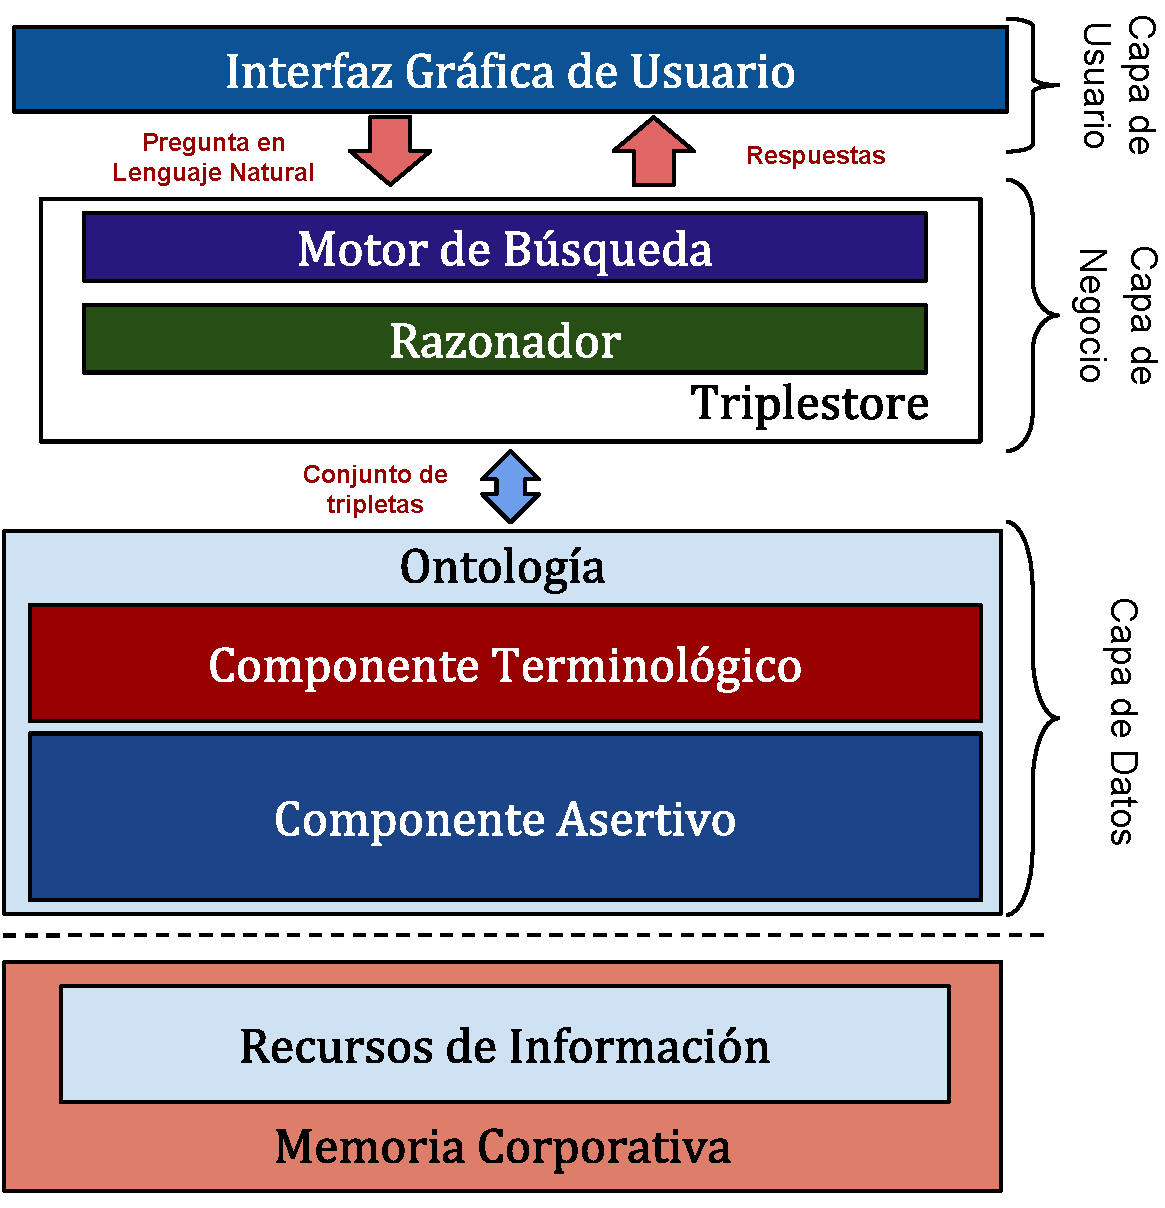
\includegraphics[scale=0.33]{Arquitectura} 
	\end{figure}
\end{frame}
%%%%%%%%%%%%%%%%%%%%%%%%%%%%%%%%%%%%%%%%%%%%%%%%%%%%%%%%%%%%%%%%%%%%%%%%%%%%%%

%%%%%%%%%%%%%%%%%%%%%%%%%%%%%%%%%%%%%%%%%%%%%%%%%%%%%%%%%%%%%%%%%%%%%%%%%%%%%%
\begin{frame}
	\frametitle{Casos de Uso}
	
	\begin{block}{}
		\begin{itemize}
		\item \justifying \textbf{\textit{Cartograf�a de Competencias}} es la b�squeda y recuperaci�n de informaci�n significativa de las personas a partir de las caracter�sticas personales y profesionales de las mismas.
		\item \justifying \textbf{\textit{B�squeda de Recursos Digitales}} es la b�squeda y recuperaci�n de informaci�n significativa de los documentos y archivos multimedia a partir del contenido de los mismos.
		\end{itemize}
	\end{block}
	
	\begin{figure}
	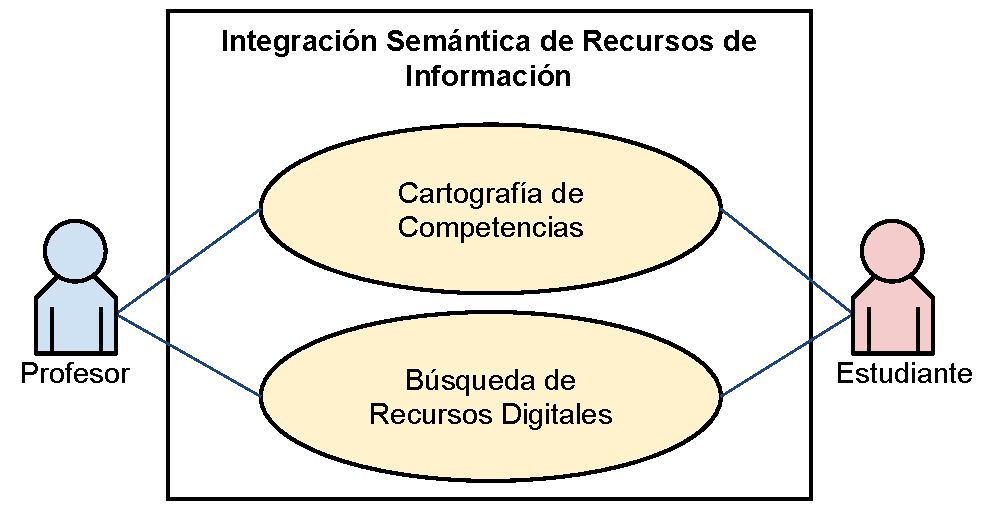
\includegraphics[scale=0.56]{CasosUso} 
	\end{figure}
\end{frame}
%%%%%%%%%%%%%%%%%%%%%%%%%%%%%%%%%%%%%%%%%%%%%%%%%%%%%%%%%%%%%%%%%%%%%%%%%%%%%%

%%%%%%%%%%%%%%%%%%%%%%%%%%%%%%%%%%%%%%%%%%%%%%%%%%%%%%%%%%%%%%%%%%%%%%%%%%%%%%
\subsection{Representaci�n el Conocimiento}
\subsubsection{Identificar los principales recursos de informaci�n}
\begin{frame}
	\frametitle{Identificar los principales recursos de informaci�n}	
	\begin{figure}
	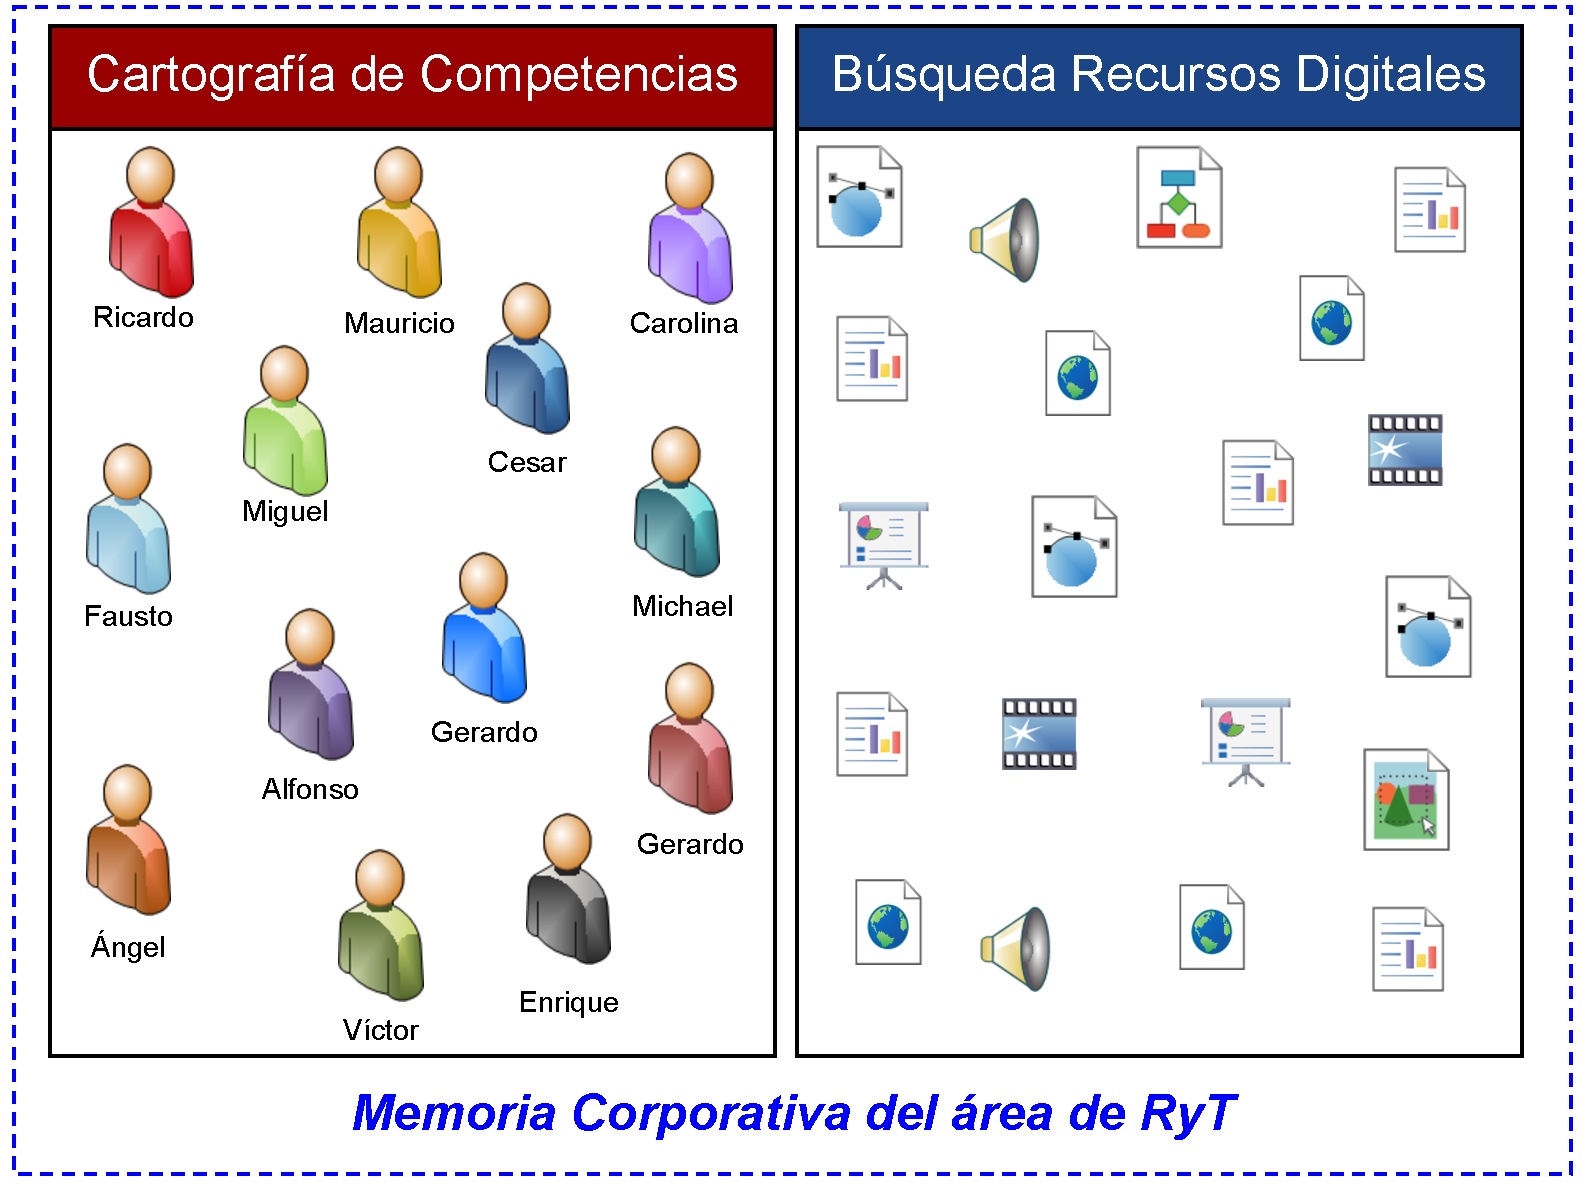
\includegraphics[scale=0.33]{CasosUsoMC} 
	\end{figure}
\end{frame}

\subsubsection{Adquirir y expresar el conocimiento de los recursos de informaci�n}
\begin{frame}
	\frametitle{Adquirir y expresar el conocimiento de los recursos de informaci�n}	
	\begin{figure}
	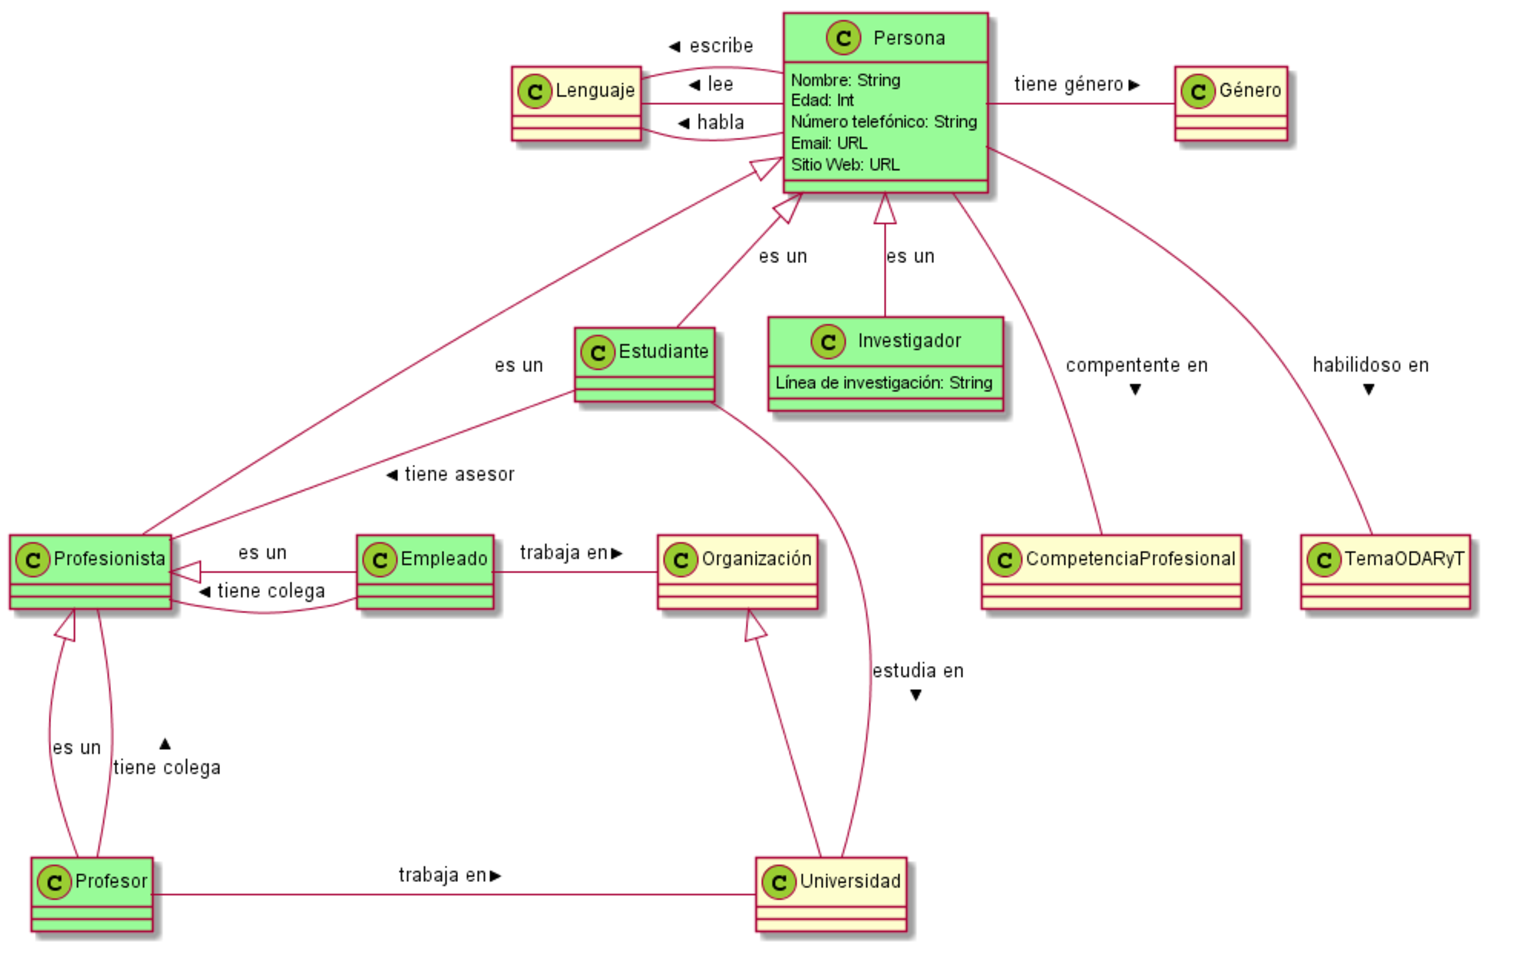
\includegraphics[scale=0.38]{CasoUsoCartComp} 
	\end{figure}
\end{frame}

\subsubsection{Representar el conocimiento e informaci�n mediante el est�ndar RDF}
\begin{frame}
	\frametitle{Representar el conocimiento e informaci�n mediante el est�ndar RDF}
	
	\begin{block}{Definici�n}
	\justifying 
	Marco gen�rico para describir el conocimiento e informaci�n expl�cita de los recursos mediante sus caracter�sticas y relaciones. \begin{scriptsize}\cite{SurvSemWeb2012}\end{scriptsize}
	\end{block}
	
	\begin{block}{Actividades en la representaci�n del conocimiento}
	\begin{enumerate}
	\item \justifying Asignar un \textit{identificador �nico de recursos} (URI) a cada \textit{recurso de informaci�n} en la \textit{memoria corporativa}.
	\item \justifying Asignar un URI a cada caracter�stica y/o relaci�n (propiedad) de de los \textit{recursos de informaci�n}.
	\item \justifying Generar las tripletas RDF asociadas a las descripciones de los recursos de informaci�n.
	\end{enumerate}
	\end{block}
%	\begin{figure}
%	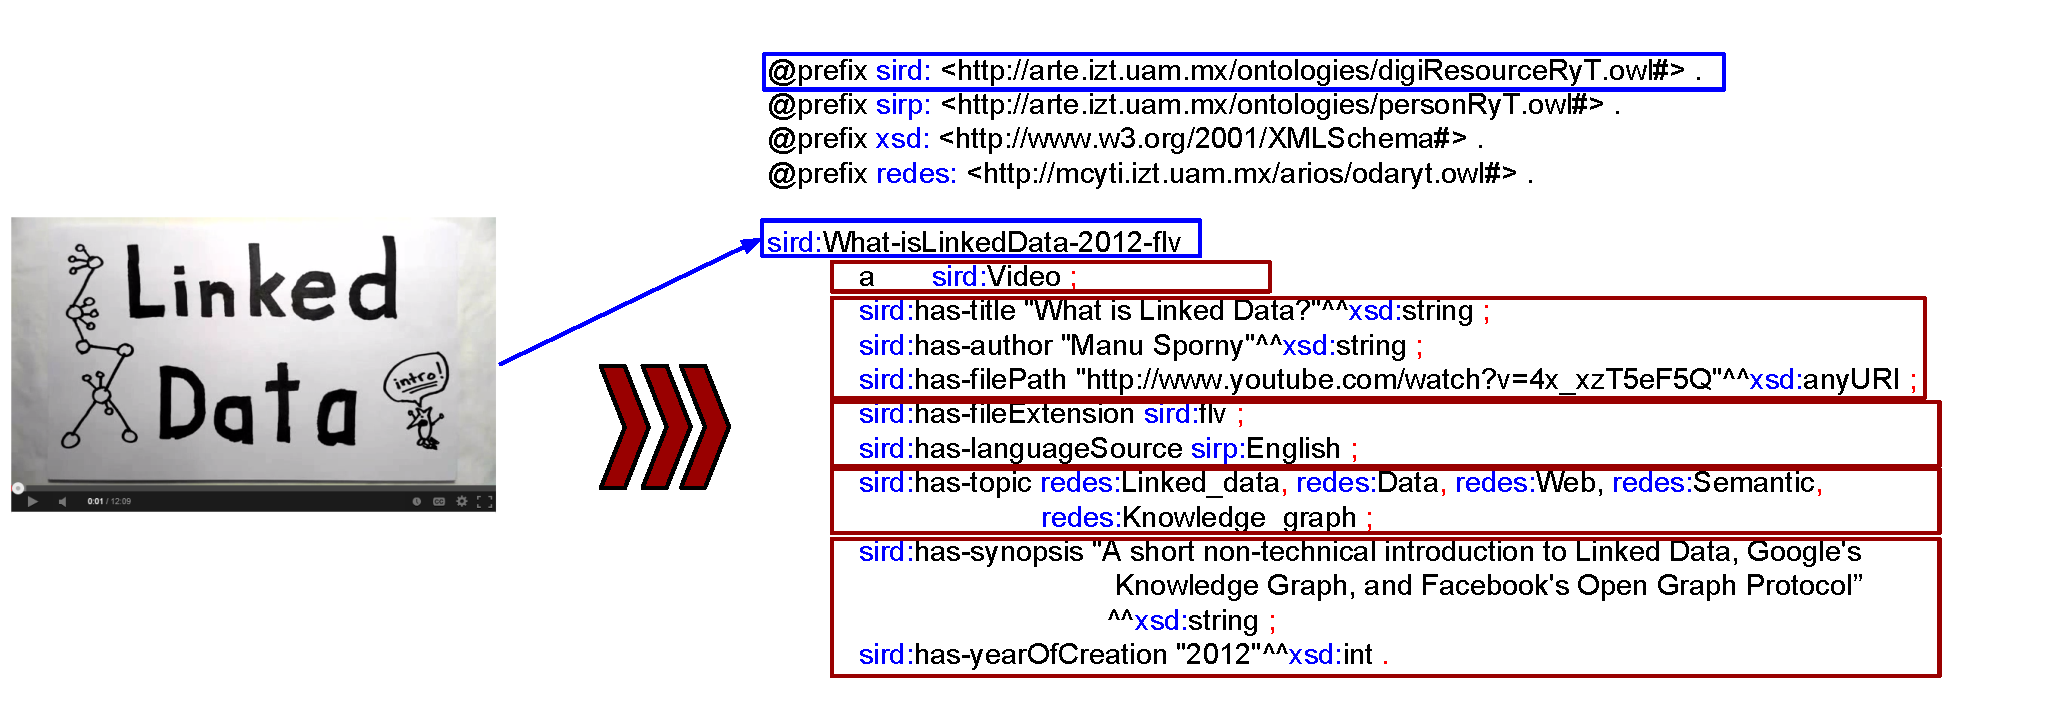
\includegraphics[scale=0.38]{Vid2RDF}
%	\end{figure}
	%%%%%%%%%%%%%%%%%%%%%%%
\end{frame}

\begin{frame}
	\frametitle{Representar el conocimiento e informaci�n mediante el est�ndar RDF}
	\begin{figure}
	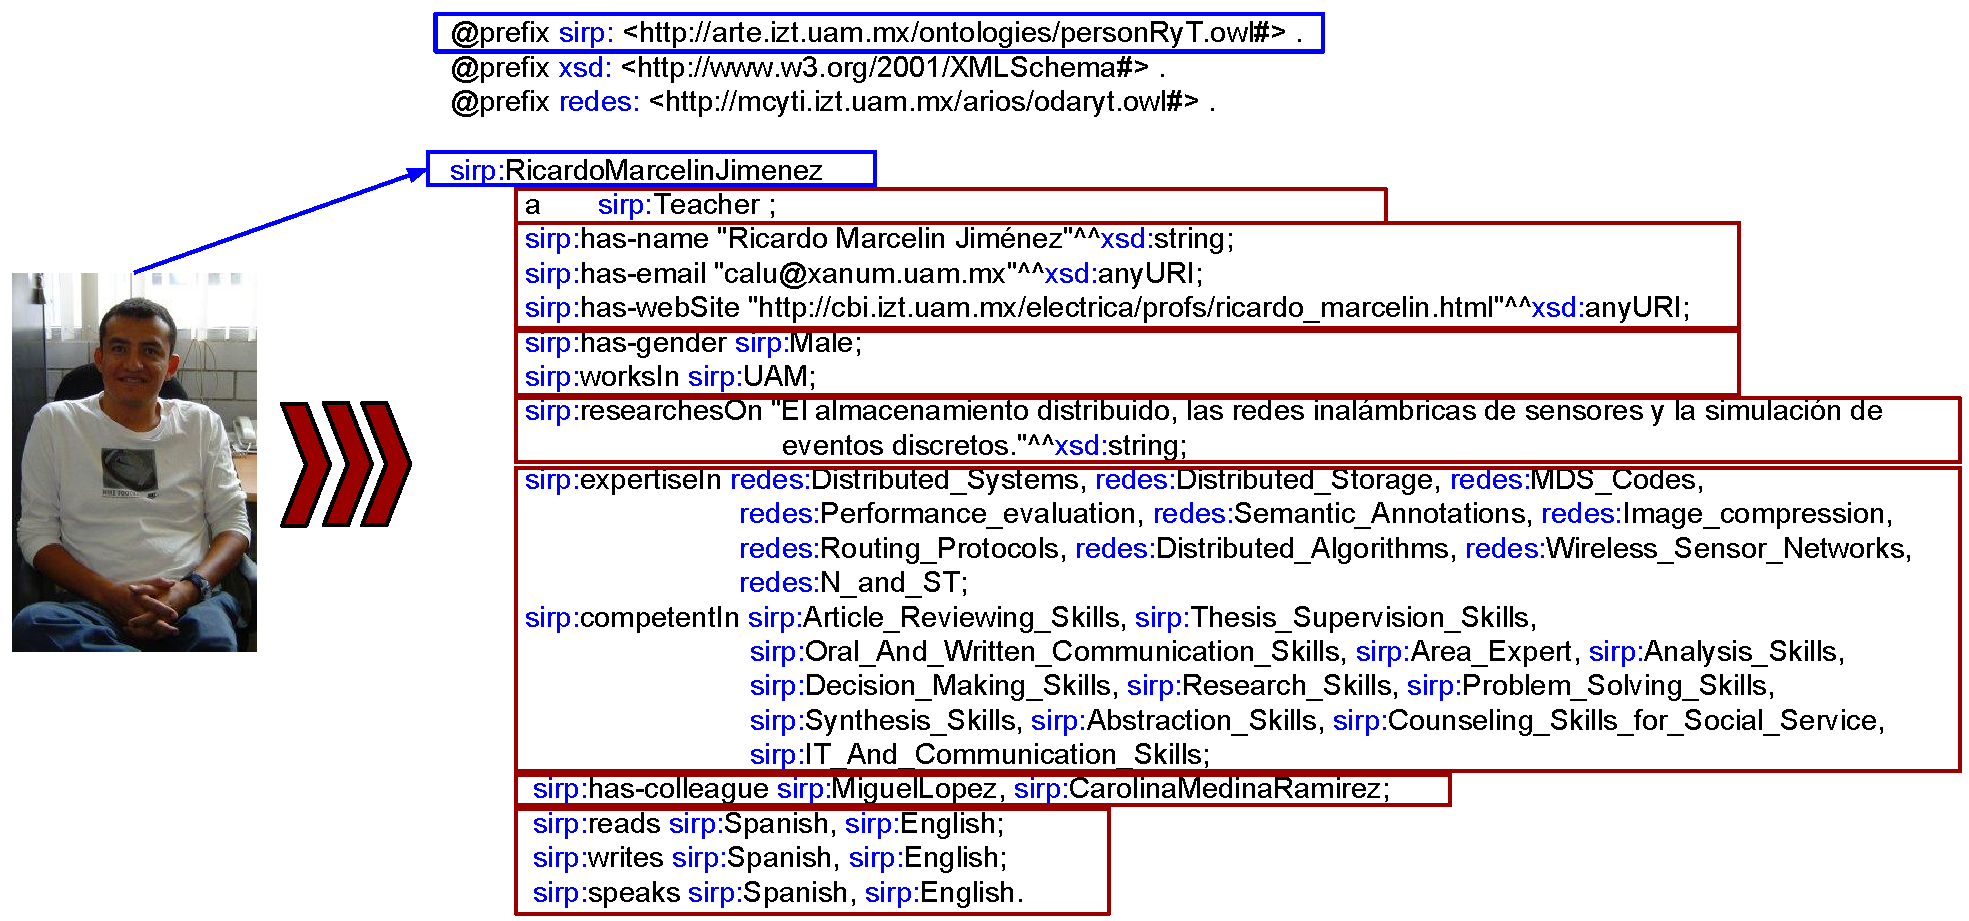
\includegraphics[scale=0.35]{Person2RDF}
	\end{figure}
\end{frame} 

\begin{frame}
	\frametitle{Representar el conocimiento e informaci�n mediante el est�ndar RDF}
	\begin{figure}
	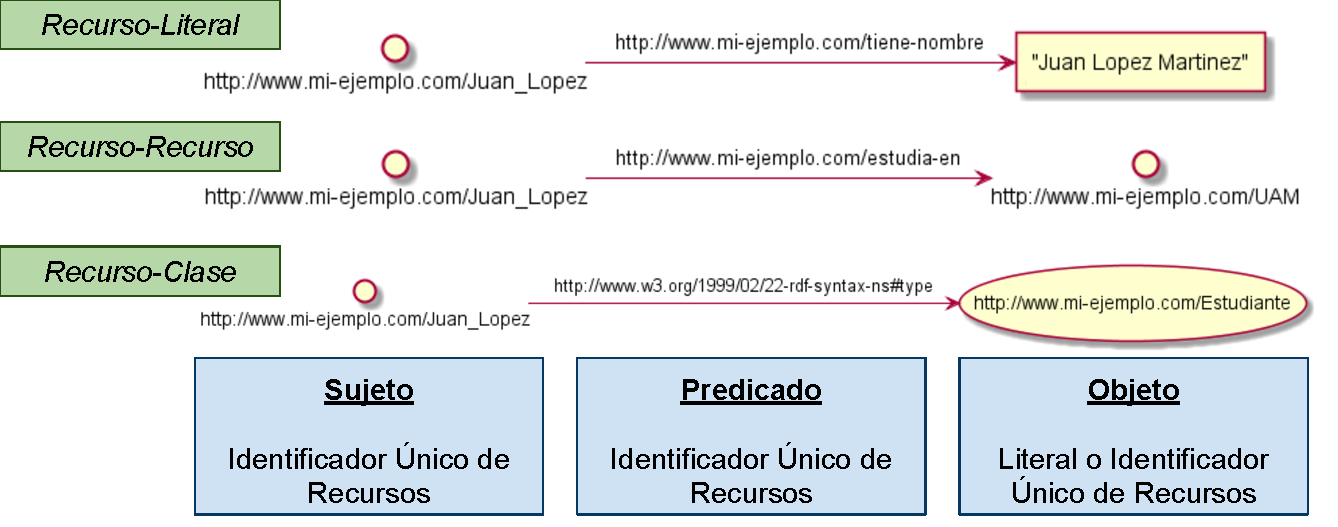
\includegraphics[scale=0.45]{Tripletas} 
	\end{figure}
\end{frame}

\begin{frame}
	\frametitle{Representar el conocimiento e informaci�n mediante el est�ndar RDF}
	\begin{figure}
	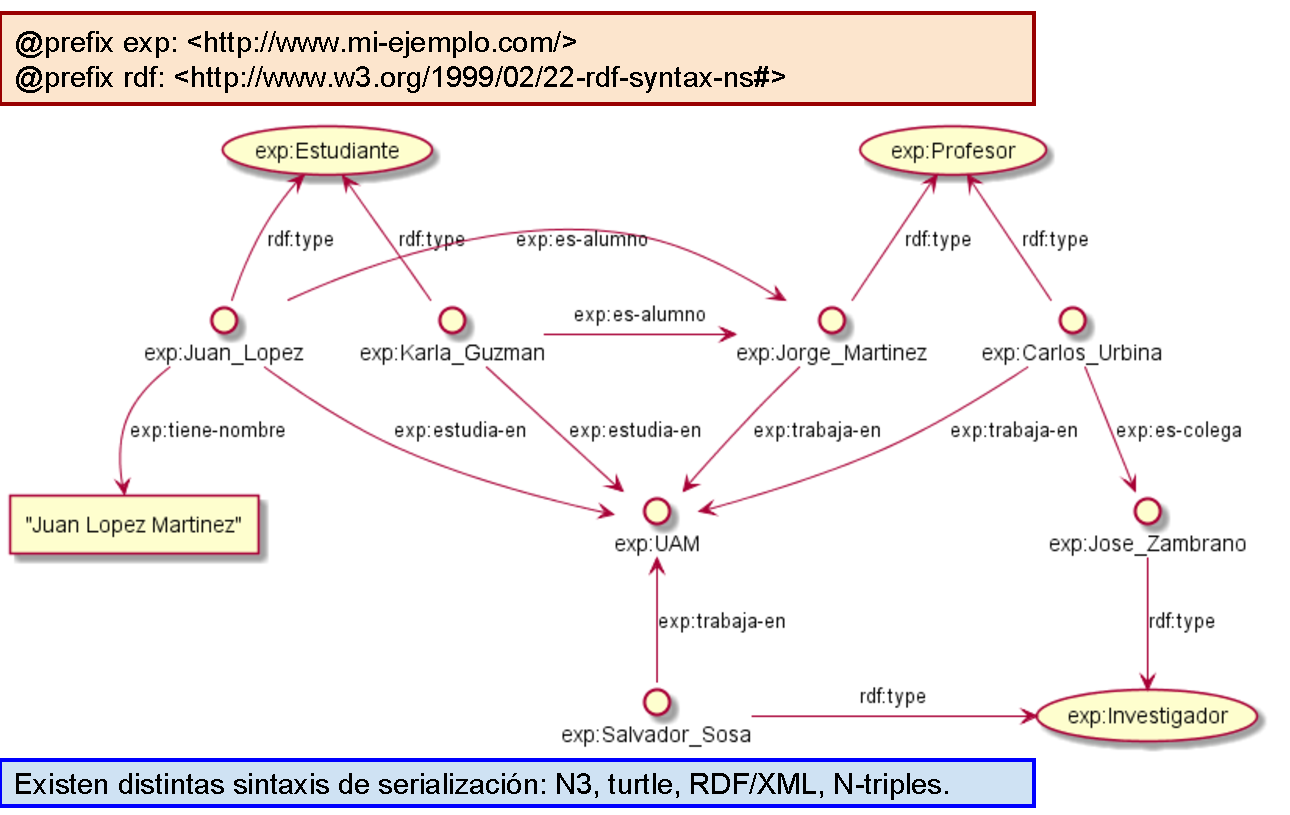
\includegraphics[scale=0.48]{GrafoRDF} 
	\end{figure}
\end{frame}

%%%%%%%%%%%%%%%%%%%%%%%%%%%%%%%%%%%%%%%%%%%%%%%%%%%%%%%%%%%%%%%%%%%%%%%%%%%%%%

\subsection{Enriquecer el conocimiento en el modelo sem�ntico}
\begin{frame}
	\frametitle{Ontolog�a}
	%%%%%%%%%%%%%%%%%%%%%%%%%%%%
	\begin{alertblock}{Definici�n}
	\justifying 
	Una definici�n formal, expl�cita y compartida de los conceptos, as� como las relaciones de un determinado dominio. \begin{scriptsize}\cite{Gruber}\end{scriptsize}
	\end{alertblock}
	
	\begin{block}{Componentes}
	\begin{itemize}
	\item \justifying \textbf{\textit{Componente Asertivo (ABox)}} est� constituido por descripciones que afirman que los individuos son instancias de una clase o propiedad.
	\item \justifying \textbf{\textit{Componente Terminol�gico (TBox)}} describe las clases y propiedades relevantes, as� como las reglas de inferencia que permiten aprovechar la manera en que las instancias se relacionan entre s�.
	\end{itemize}
	\end{block}
	%%%%%%%%%%%%%%%%%%%%%%%%%%%%
\end{frame}

\begin{frame}
	\frametitle{Axiomatizaci�n}	
	\begin{block}{Reglas de inferencia o Axiomas}
	\justifying 
	Expresiones para enriquecer un grafo RDF con conocimiento impl�cito.\\
	\end{block}
	
	\begin{block}{Lenguajes}
	Especificaciones para describir clases, propiedades e individuos.
	\begin{itemize}
	\item \justifying \textit{RDF Schema \textbf{RDF(S)}}
	\item \justifying \textit{Web Ontology Language \textbf{OWL}} 
	\end{itemize}
	\end{block}
	
	\begin{figure}
	
\includegraphics[scale=0.4]{PrefijosRDFSOWL}
	\end{figure}
	
	\begin{block}
	\justifying
	\textit{Lo que es obvio para un humano, no lo es para una maquina}.
	\end{block}
\end{frame}

%\begin{frame}
%	\frametitle{Enriquecer el conocimiento en el modelo sem�ntico}
%	\begin{block}{}
%	\justifying
%	Para cada \textit{caso de uso} debe encontrarse el respectivo conjunto de axiomas (TBox).
%	\end{block}
%	
%	\begin{figure}
%	
\includegraphics[scale=0.4]{PrefijosRDFSOWL}
%	\end{figure}
%\end{frame}
	
\subsubsection{Herencia de Clases}
\begin{frame}[allowframebreaks]
	\frametitle{Herencia de Clases}
	\begin{block}{Subclase (rdfs:subClassOf)}
	\justifying
	Afirma que una \textit{clase A} se subsume por una \textit{clase B}, es decir, la clase A es un caso particular de la \textit{clase B}. En este caso, las instancias de la clase A son instancias de la clase B.
	\end{block}
	
	\begin{figure}
	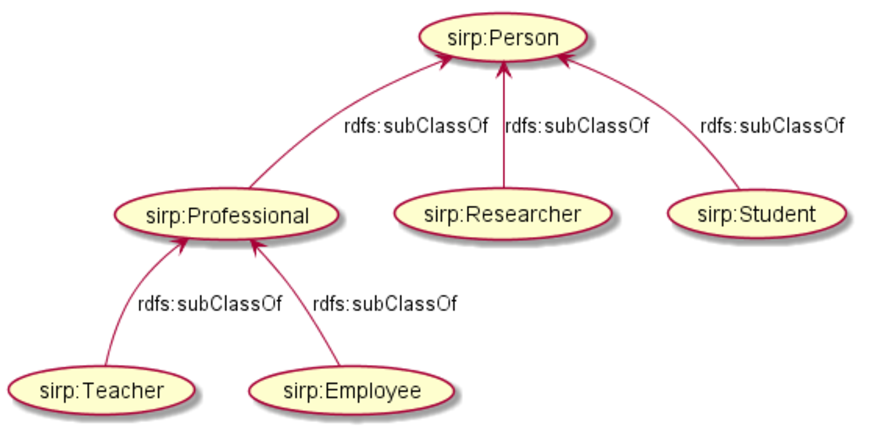
\includegraphics[scale=0.5]{HerenClassCartComp}
	\end{figure}
	%%%%%%%%%%%%%%%%%%%%%%%
	
	\begin{figure}
	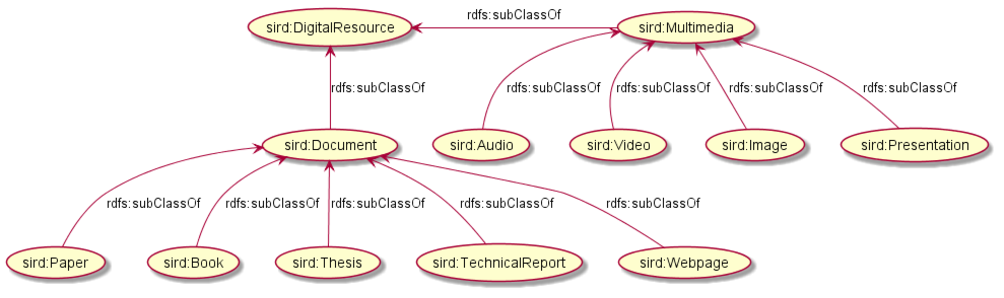
\includegraphics[scale=0.68]{HerenClassRecDigi}
	\end{figure}
	%%%%%%%%%%%%%%%%%%%%%%%
	
	\begin{figure}
	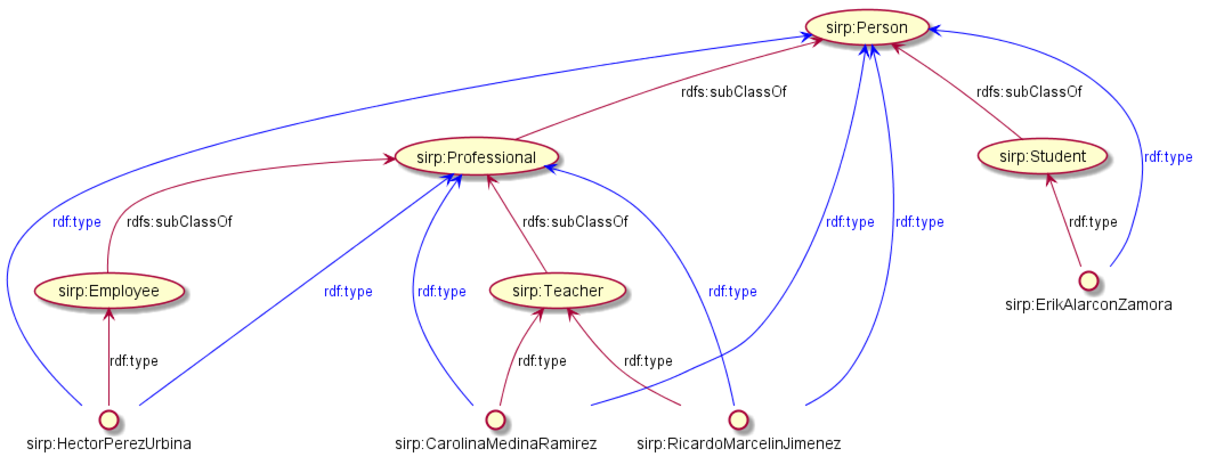
\includegraphics[scale=0.57]{EjmpInfSubClass}
	\end{figure}
	%%%%%%%%%%%%%%%%%%%%%%%
\end{frame}

\subsubsection{Herencia de Propiedades}
\begin{frame}[allowframebreaks]
	\frametitle{Herencia de Propiedades}
	\begin{block}{Subpropiedad (rdfs:subPropertyOf)}
	\justifying
	Afirma que todos los recursos que se relacionan por la \textit{propiedad X}, tambi�n se relacionan por la \textit{propiedad Y}.
	\end{block}
	
	\begin{figure}
	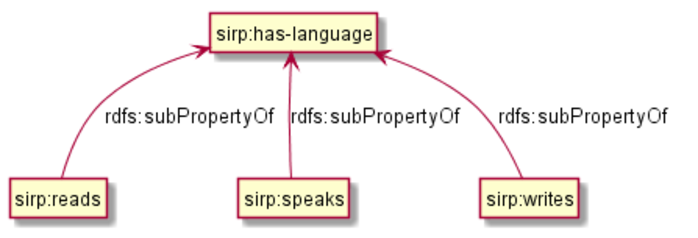
\includegraphics[scale=0.57]{HerPropLang}
	\end{figure}
		
	\begin{figure}
	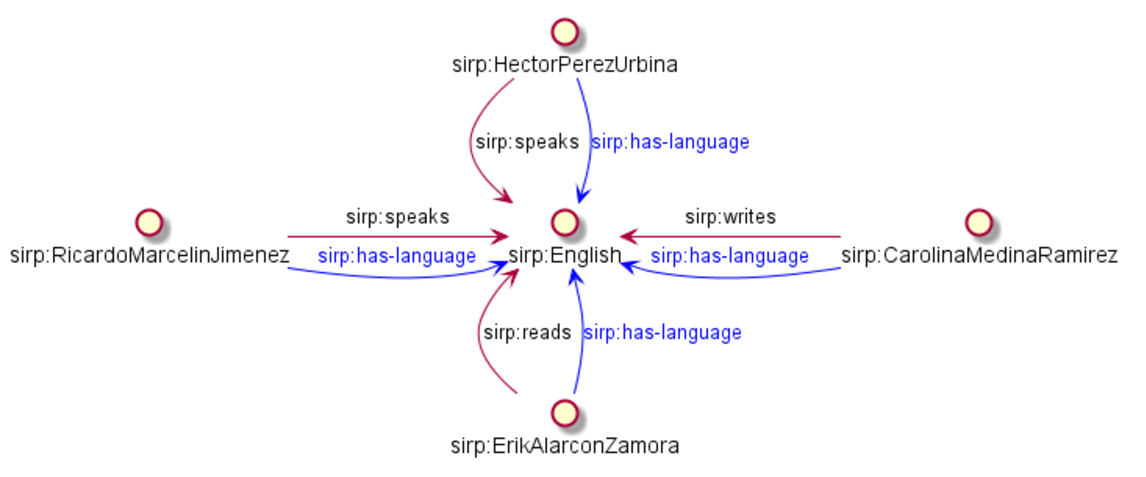
\includegraphics[scale=0.55]{EjmpInfProp}
	\end{figure}
	%%%%%%%%%%%%%%%%%%%%%%%
\end{frame}

\subsubsection{Dominio y Rango en las Propiedades}
\begin{frame}[allowframebreaks]
	\frametitle{Dominio y Rango en las Propiedades}
	\begin{block}{Dominio (rdfs:domain)}
	\justifying
	Especifica qu� clase se aplica a una propiedad.
	\end{block}
	
	\begin{block}{Rango (rdfs:range)}
	\justifying
	Especifica los valores (clase o tipo de literal) que puede asumir una propiedad.
	\end{block}
	
	\begin{figure}
	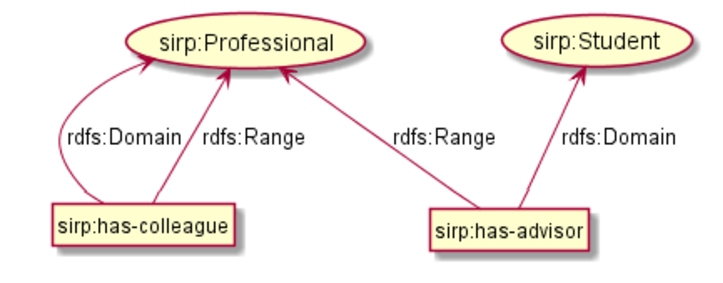
\includegraphics[scale=0.52]{exAxDyRPer}
	\end{figure}
	%%%%%%%%%%%%%%%%%%%%%%%
	
	\begin{figure}
	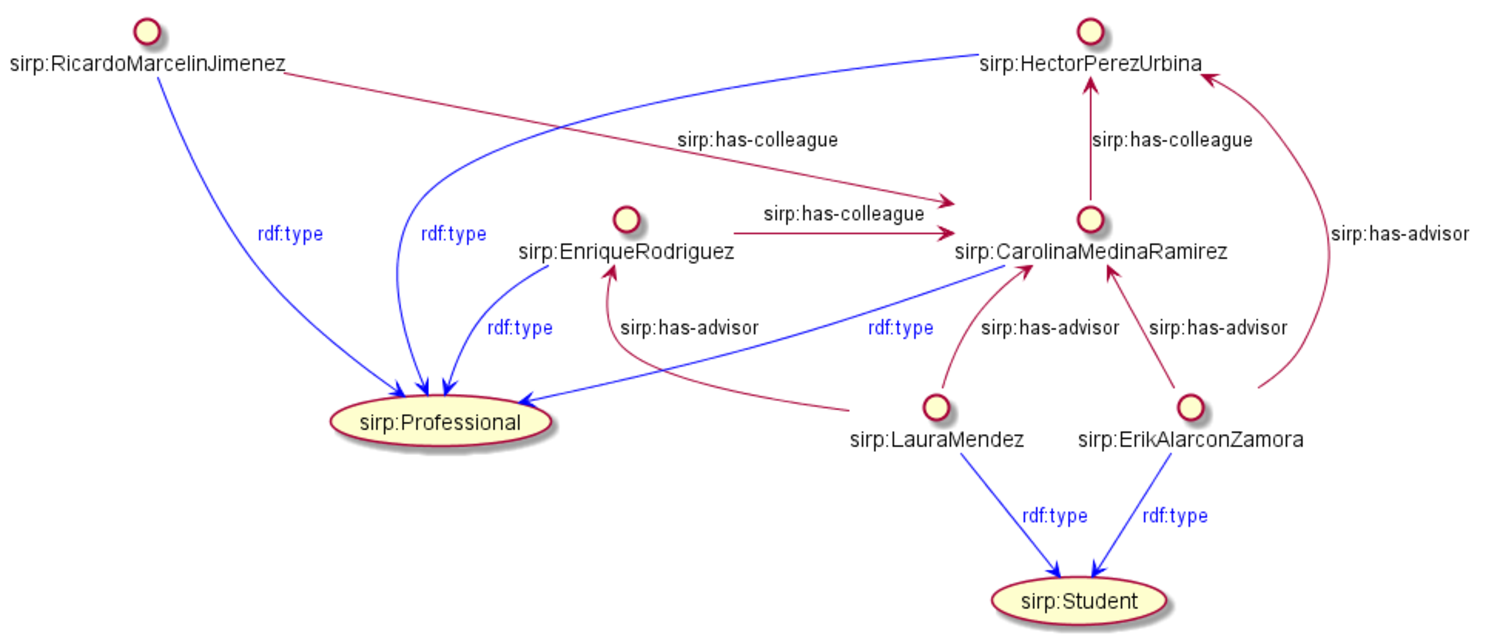
\includegraphics[scale=0.45]{exInfDyRPer}
	\end{figure}
	%%%%%%%%%%%%%%%%%%%%%%%
\end{frame}

\subsubsection{Caracter�sticas en las Propiedades}
\begin{frame}
	\frametitle{Caracter�sticas en las propiedades}
	\begin{block}{Propiedad sim�trica (owl:SymmetricProperty)}
	\justifying
	Afirma que la \textit{propiedad X} es su propia propiedad inversa, es decir, si la \textit{propiedad X} relaciona al \textit{individuo A} con el \textit{individuo B}, entonces, esta propiedad debe relacionar al \textit{individuo B} con el \textit{individuo A}.
	\end{block}
	
	\begin{figure}
	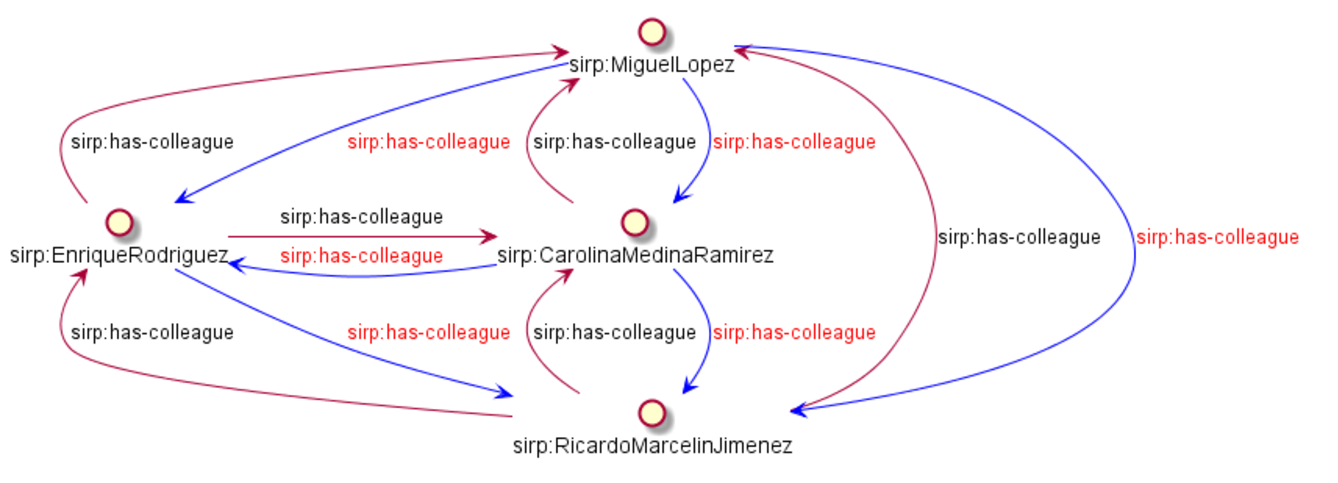
\includegraphics[scale=0.5]{infSymColl}
	\end{figure}
	%%%%%%%%%%%%%%%%%%%%%%%
\end{frame}
%%%%%%%%%%%%%%%%%%%%%%%%%%%%%%%%%%%%%%%%%%%%%%%%%%%%%%%%%%%%%%%%%%%%%%%%%%%%%%

\subsection{Buscar y recuperar la informaci�n en el modelo sem�ntico}
\begin{frame}
	\frametitle{Buscar y recuperar la informaci�n en el modelo sem�ntico}
%	\begin{block}{Objetivo}
%	\justifying
%	La b�squeda y recuperaci�n de la informaci�n para responder las preguntas o necesidades informativas de los usuarios del �rea de Redes y Telecomunicaciones (RyT).
%	\end{block}
	
	\begin{block}{SPARQL}
	\justifying 
	Lenguaje de consulta y protocolo de acceso a RDF, para la b�squeda y recuperaci�n de la informaci�n en un grafo RDF.
	\end{block}
	
	\begin{figure}
	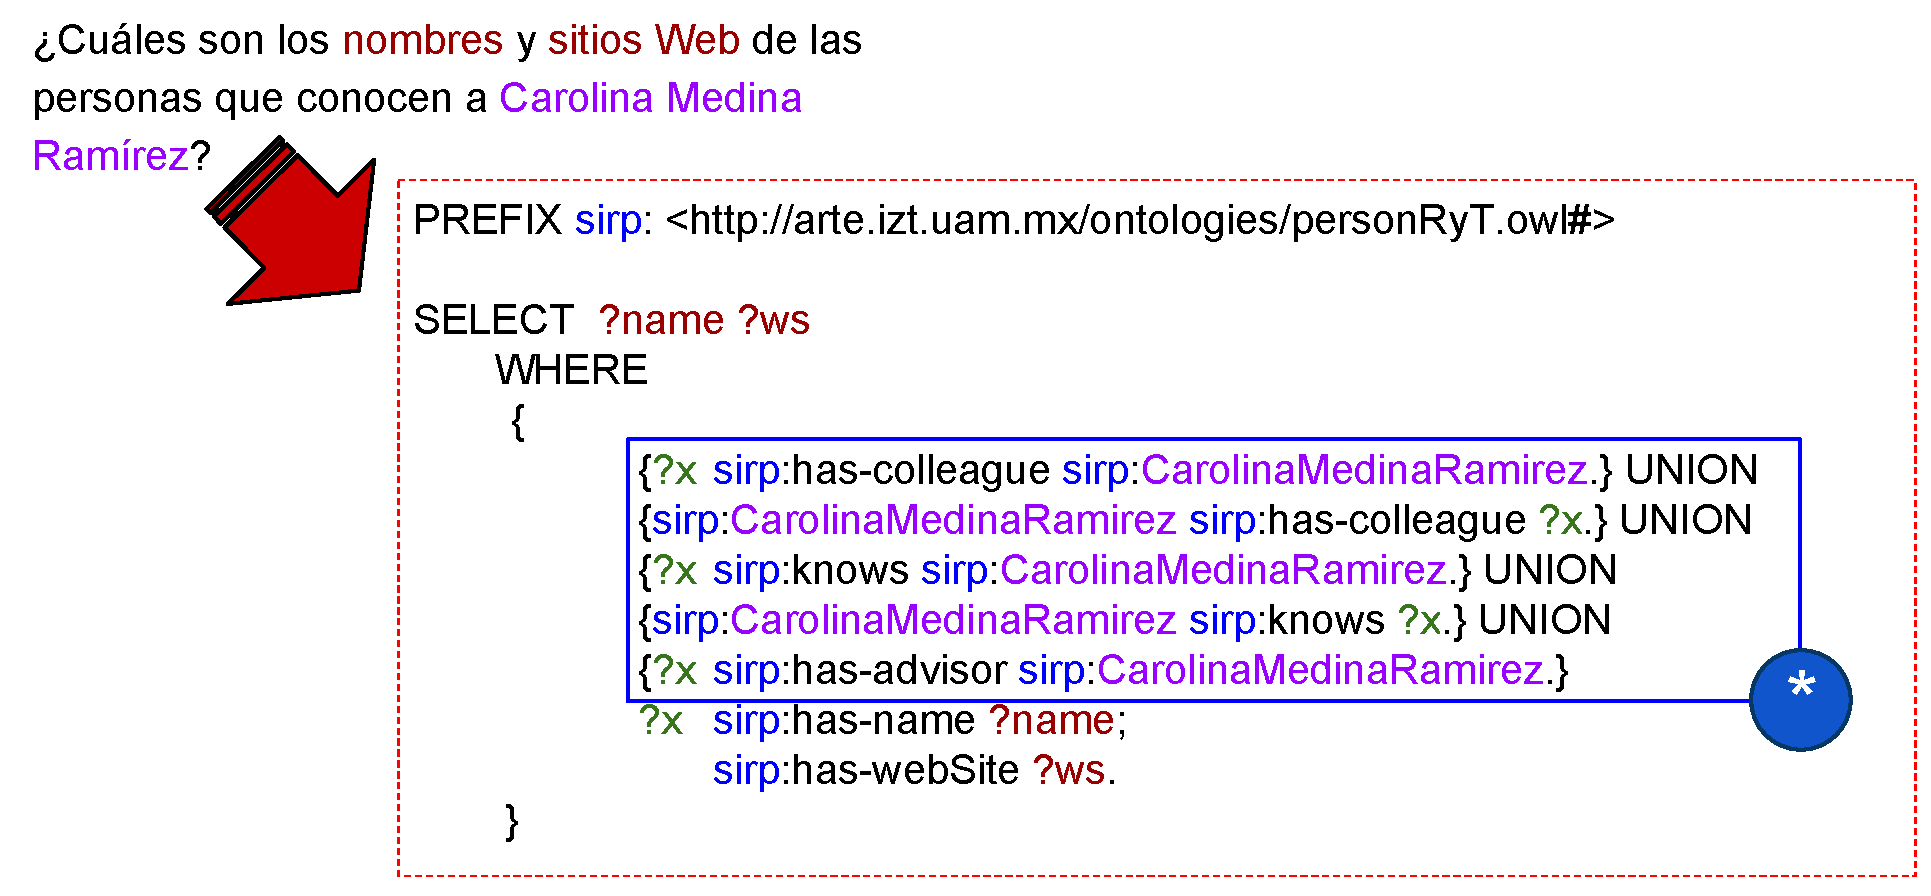
\includegraphics[scale=0.32]{q2rqlSR}
	\end{figure}
	
%	\begin{block}{Actividades}
%	\begin{enumerate}
%	\item \justifying Identificar las preguntas en lenguaje natural.
%	\item \justifying Transformar las preguntas a una consultas SPARQL.
%	\item \justifying Ejecutar las consultas mediante un motor de b�squeda SPARQL.
%	\end{enumerate}
%	\end{block}

\end{frame}

%%%%%%%%%%%%%%%%%%%%%%%%%%%%%%%%%%%%%%%%%%%%%%%%%%%%%%%%%%%%%%%%%%%%%%%%%%%%%%
\subsubsection{B�squeda + Inferencia}
\begin{frame}[allowframebreaks]
	\frametitle{Uso de inferencia}
		
	\begin{figure}
	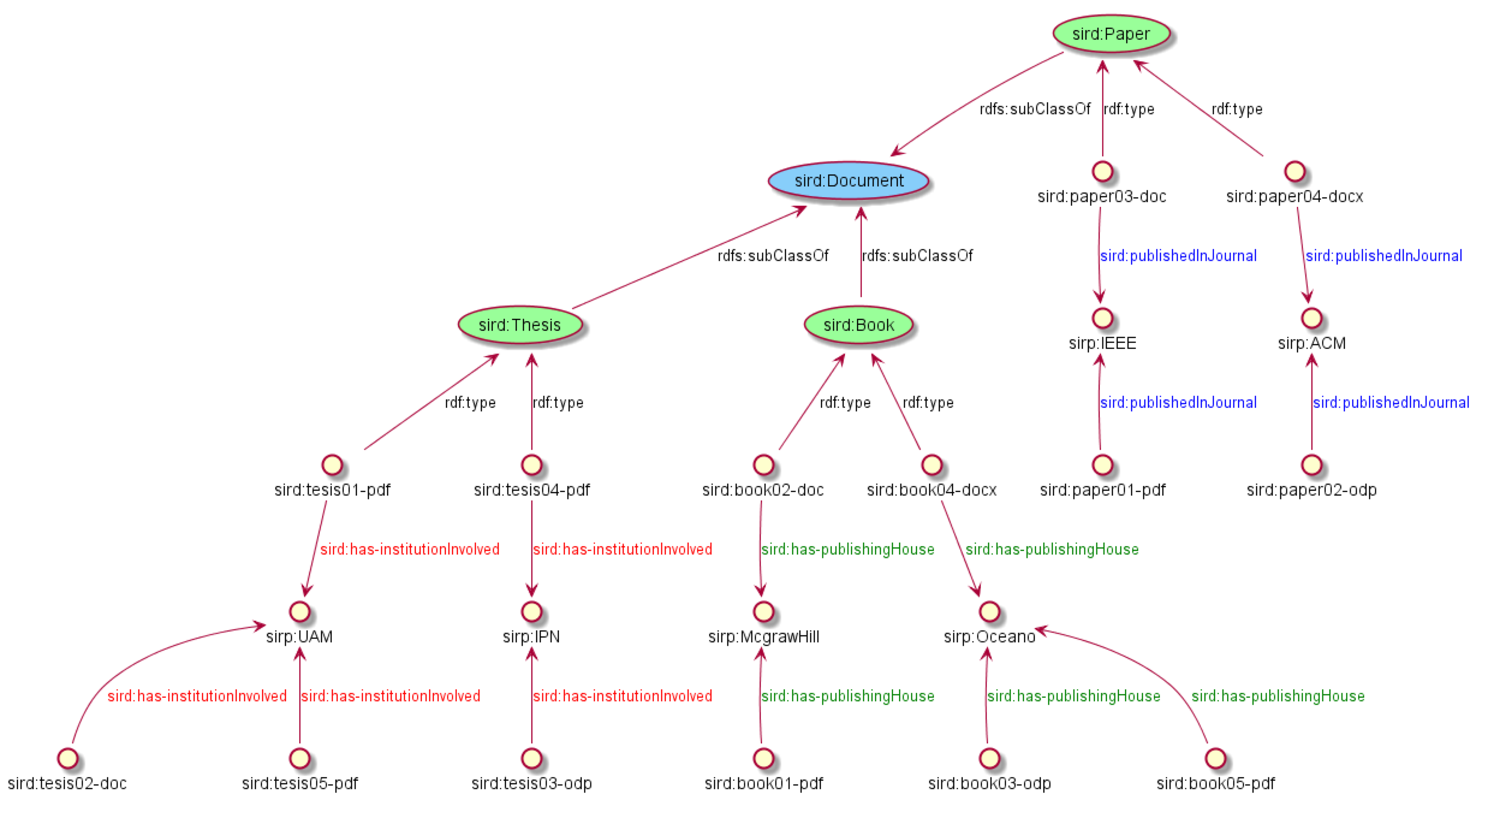
\includegraphics[scale=0.3]{grafoSR}
	\caption{Grafo RDF sin inferencia}
	\end{figure}
	%%%%%%%%%%%%%%%%%%%%%%%%%%%%%%%%%%%
	
	\begin{figure}[htbp]
	\centering
	\subfigure[Consulta sin inferencia]{
	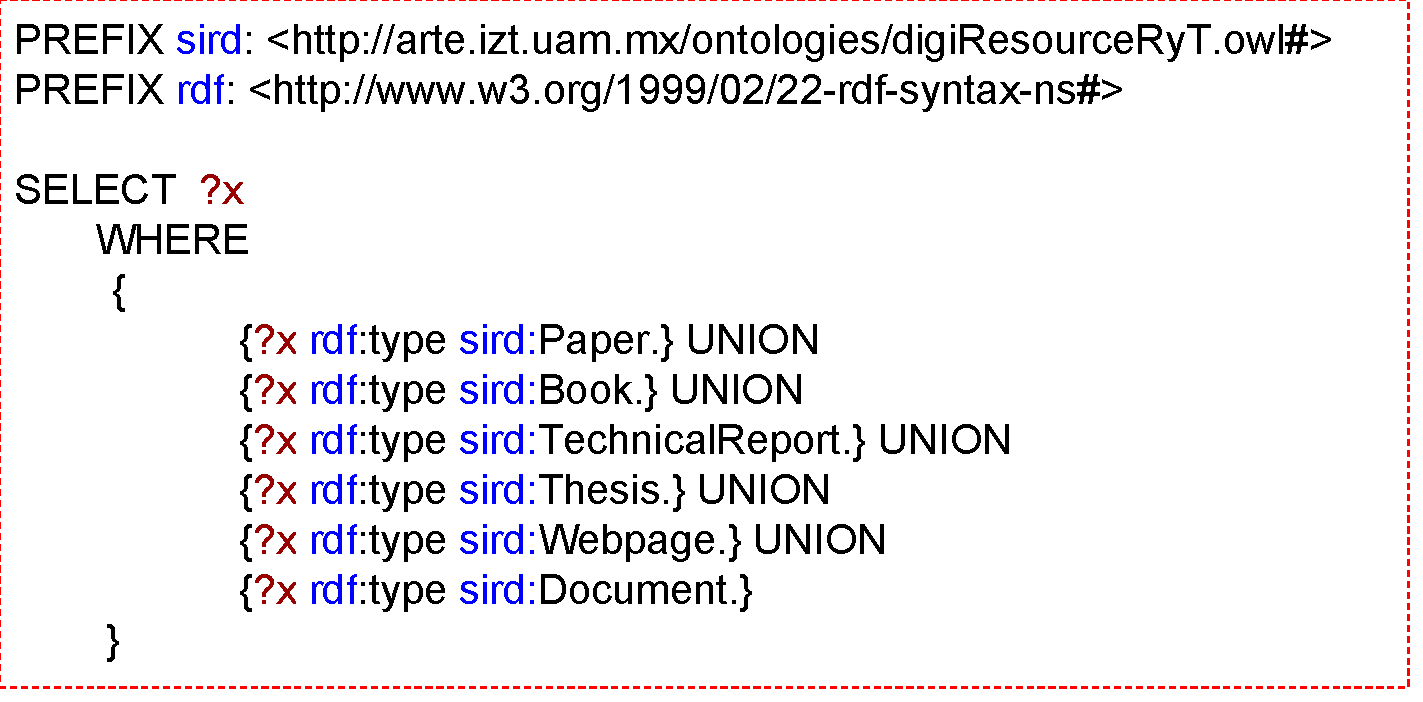
\includegraphics[scale=0.25]{consultaGrafo} 
	}
	\subfigure[Resultados de la consulta]{
	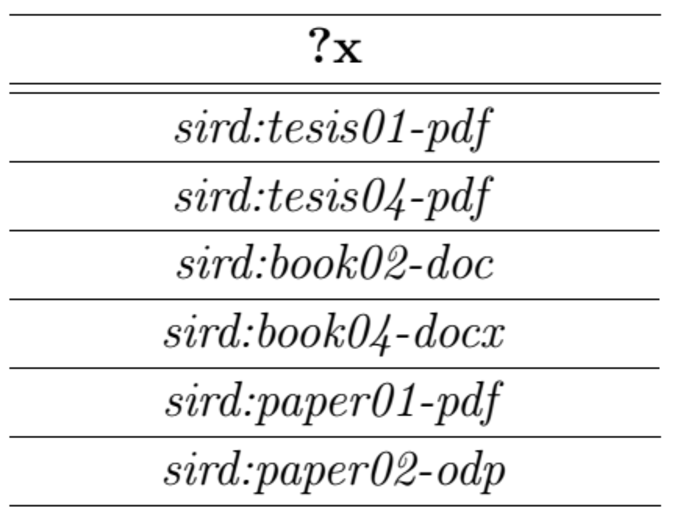
\includegraphics[scale=0.28]{RespQrySI} 
	}
	\end{figure}
	%%%%%%%%%%%%%%%%%%%%%%%%%%%%%%%%%%%
	
	\begin{figure}
	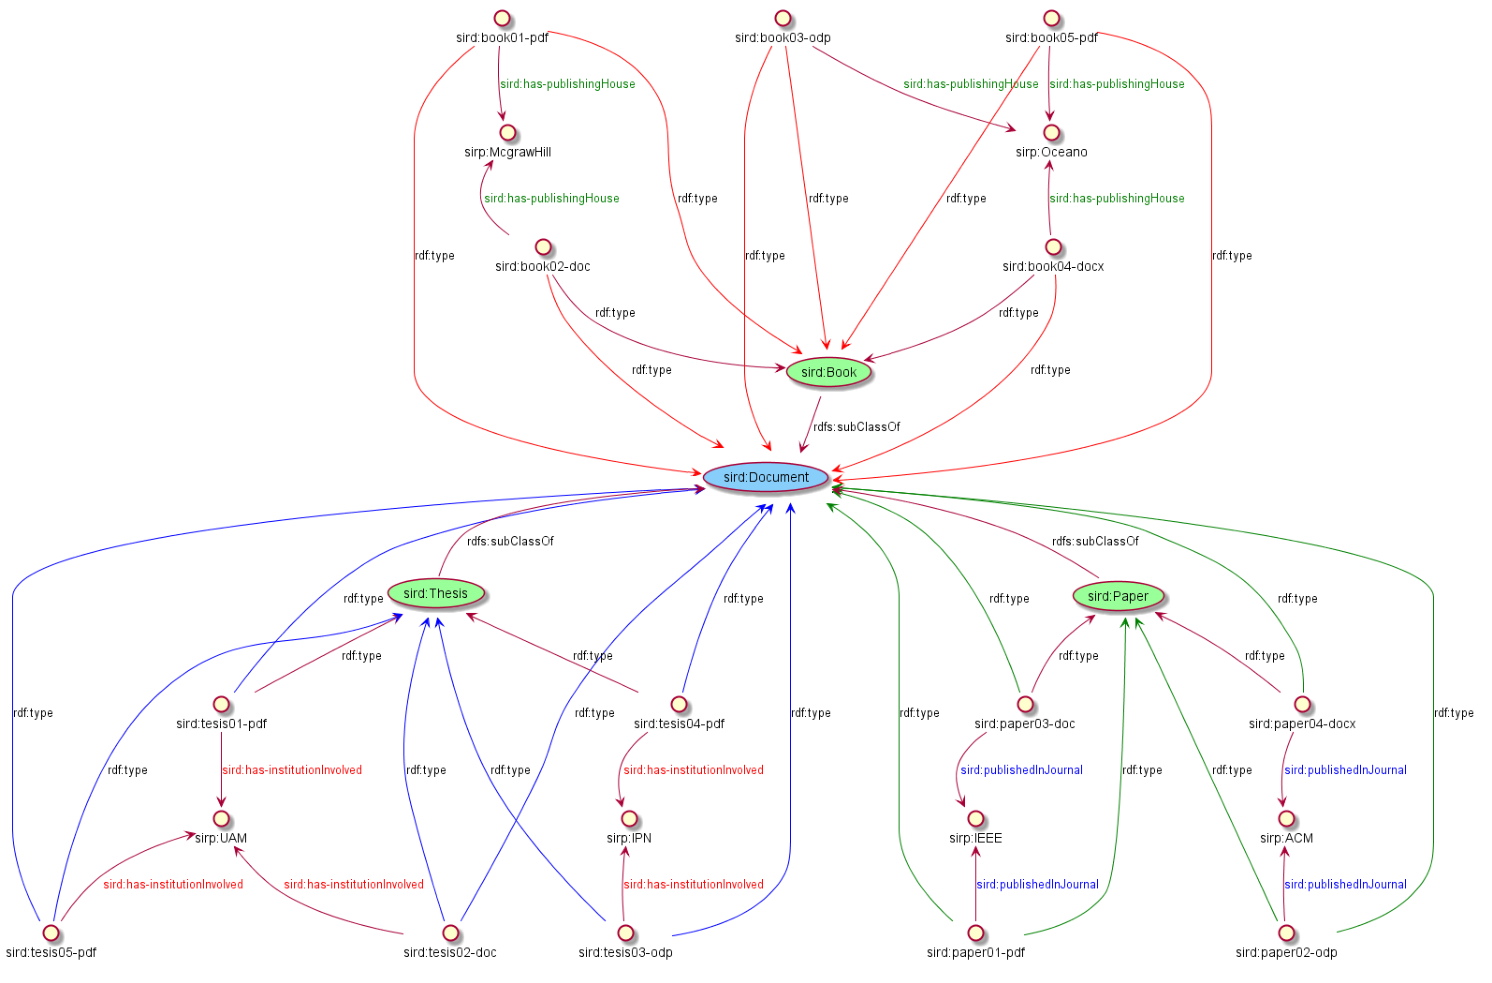
\includegraphics[scale=0.37]{grafoCR}
	\caption{Grafo RDF con inferencia}
	\end{figure}	
	%%%%%%%%%%%%%%%%%%%%%%%%%%%%%%%%%%%
\end{frame}

\subsubsection{Uso de inferencia IV}
\begin{frame}
	\frametitle{Uso de inferencia IV}
	\begin{figure}[htbp]
	\centering
	\subfigure[Consulta con inferencia]{
	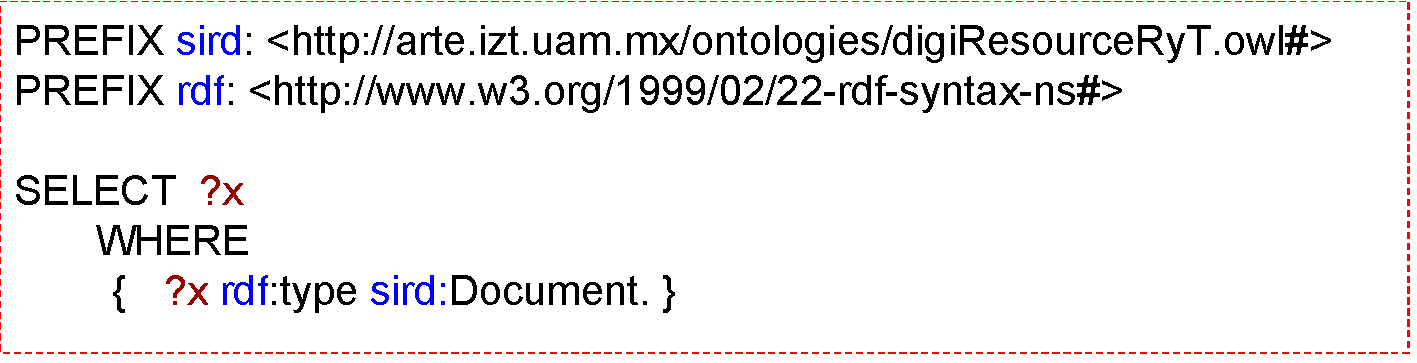
\includegraphics[scale=0.25]{consSimpGrafo} 
	}
	\subfigure[Resultados de la consulta]{
	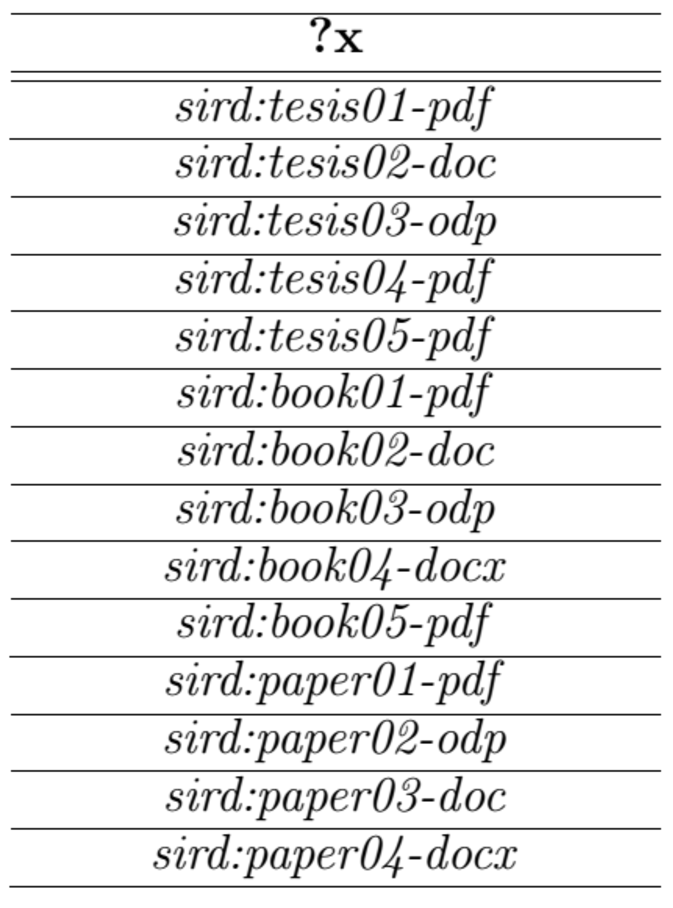
\includegraphics[scale=0.28]{RespQryCI} 
	}
	\end{figure}
\end{frame}
\chapter{Prototipo}
\label{cap:piu}
%%No solo basta con un razonador también se requiere un modulo integrador de la información que transforme las consultas de los usuarios expresadas en lenguaje natural, a lenguaje que sea interpretado por el razonador. Además este integrador es el encargado de regresar los enlaces y los datos del recurso. De esta manera el motor de búsqueda queda de la siguiente manera:

%%Para llevar acabo está integración de la información es necesario un prototipo que satisfaga más eficientemente las consultas que escribe el usuario. De esta manera es necesario un análisis documental y técnico de los módulos de Anotaciones, Ontología de Dominio y Razonadores. Con la finalidad de tener una propuesta de sistema con las últimas novedades hechas en búsqueda y recuperación de la información basada en la semántica de los recursos.

%%se requiere proporcionar interfaces fáciles de usar, para simplificar a los miembros el proceso de generación de anotaciones y colocar en contexto su trabajo.  Un buen enfoque para un sistema de anotaciones es aquel donde se maneja una única interfaz, y es en esta donde los usuarios crean, modifican y comparten sus anotaciones.

%%La interfaz debe tener ..., para que los usuarios estructuren sus consulta, capturando los valores que desean buscar. En la interfaz debe proporcionar un navegador entre personas, documentos, multimedia, para que los usuarios que no tienen algún conocimiento previo de las personas y recursos digitales, puedan tener una vision general de la información de los recursos.

%%La interfaz debe permitir hacer las siguientes actividades a los usuarios:
%%•	Login.
%%•	Navegar entre personas.
%%o	Filtrar por ocupación.
%%o	Mostrar la información más detallada de una persona.
%%o	Búsqueda Avanzada de las personas.
%%•	Navegar entre documentos.
%%o	Filtrar por clase de documento.
%%o	Mostrar la información más detallada de un documento.
%%o	Búsqueda Avanzada de documentos.
%%•	Navegar entre multimedia.
%%o	Filtrar por clase multimedia.
%%o	Mostrar la información más detallada de un recurso multimedia.
%%o	Búsqueda Avanzada de recursos multimedia.
%%•	Búsqueda en todos los recursos de información por información semejante.

%%Las distintas aplicaciones que hay pueden ser elaboradas para Windows, Linux, Macs, u otros sistemas operativos, y también se pueden tener distintas versiones del mismo sistema para poder trabajar entre los distintos sistemas operativos. Lo ideal es que sin importar cual sea el sistema operativo el usuario pueda realizar sus anotaciones semánticas, para logara esto se puede emplear una aplicación web o aplicaciones elaboradas en java.
%%Si se emplea una aplicación web no es necesario instalar algún software extra, solo basta que el usuario acceda utilizando su navegador web de preferencia y comience el proceso de creación de anotaciones semánticas.

%%Por otro lado al usar una aplicación basada en Java, es necesario tener Java Development Kit (JDK) que es independiente de la plataforma, para tener un entorno amigable al usuario.

%%Finalmente, los usuarios necesitan una interfaz de usuario, para la consulta de información de las tripletas. Nosotros proponemos una interfaz amigable que sea accesible vía Web. De esta manera, los usuarios no instalan ningún componente y simplemente acceden a la página Web del sistema.
%%La interfaz al ser accesible vía Web, requiere ser instalada en un servidor Web. Para tomar la decisión sobre qué servidor es el apropiado para la interfaz. Nosotros debemos tomar en cuenta, el lenguaje de implementación del triplestore. Si el lenguaje es PHP9, entonces, podemos emplear un servidor HTTP Apache10. En otro caso, si el lenguaje es Java11 y permite implementar Servlet, entonces el servidor es Apache Tomcat12. 



\section{Referencias}
\begin{frame}[allowframebreaks]
\frametitle{Referencias}
\begin{scriptsize} \bibliographystyle{apalike}
\justifying \bibliography{bibliografia}\end{scriptsize}
\end{frame}

\end{document}
